\documentclass[11pt,a4paper,openany]{book}
\usepackage[T1]{fontenc}
\usepackage[utf8]{inputenc}
\usepackage{lmodern}
\usepackage{microtype}
\usepackage[a4paper,margin=24mm,headheight=15pt]{geometry}
\usepackage{xcolor}
\usepackage{graphicx}
\usepackage{booktabs}
\usepackage{tabularx}
\usepackage{longtable}
\usepackage{array}
\usepackage{enumitem}
\usepackage{listings}
\usepackage[most]{tcolorbox}
\usepackage{tikz}
\usetikzlibrary{arrows.meta,positioning,calc,shapes.geometric,fit}
\usepackage{fancyhdr}
\usepackage{titlesec}
\usepackage{hyperref}
\usepackage{bookmark}
\usepackage{xurl}
\usepackage{amsmath}
\usepackage{amssymb}
\usepackage{textcomp}
\usepackage[strings]{underscore}
\usepackage{lastpage}

\definecolor{FarmGreen}{HTML}{2F5D50}
\definecolor{FarmGreenLight}{HTML}{EAF2EF}
\definecolor{FarmGold}{HTML}{B38A3E}
\definecolor{FarmGoldLight}{HTML}{FBF5E8}
\definecolor{FarmRed}{HTML}{8E3B32}
\definecolor{FarmBlue}{HTML}{365F7A}
\definecolor{Ink}{HTML}{202625}
\definecolor{Muted}{HTML}{5D6965}
\definecolor{CodeBg}{HTML}{F6F7F6}
\definecolor{CodeBorder}{HTML}{D9DEDB}
\definecolor{WarnBg}{HTML}{FFF3E5}
\definecolor{InfoBg}{HTML}{EEF5FA}
\definecolor{EditBg}{HTML}{EEF7EF}

\hypersetup{
  colorlinks=true,
  linkcolor=FarmGreen,
  urlcolor=FarmBlue,
  citecolor=FarmRed,
  pdftitle={Willowfield - Complete Beginner Codebase Handbook},
  pdfauthor={Sivothayan .S},
  pdfsubject={Beginner codebase architecture, customization, build, testing, and modification guide for the Willowfield interactive 3D farm project},
  pdfkeywords={Willowfield, CSC3081, C++20, OpenGL, FreeGLUT, computer graphics, 3D farm, codebase handbook, source code documentation, software architecture, procedural animation, vegetation, CMake}
}

\setlist[itemize]{topsep=3pt,itemsep=2pt,leftmargin=1.5em}
\setlist[enumerate]{topsep=3pt,itemsep=2pt,leftmargin=1.8em}
\renewcommand{\arraystretch}{1.18}

\pagestyle{fancy}
\fancyhf{}
\fancyhead[LE]{\small\color{Muted}\leftmark}
\fancyhead[RO]{\small\color{Muted}\rightmark}
\fancyfoot[C]{\small\color{Muted}Willowfield Codebase Handbook -- Page \thepage}
\renewcommand{\headrulewidth}{0.3pt}
\renewcommand{\footrulewidth}{0pt}

\titleformat{\chapter}[display]
  {\normalfont\huge\bfseries\color{FarmGreen}}
  {\filleft\Large\color{FarmGold}\chaptertitlename\ \thechapter}
  {1ex}
  {\titlerule\vspace{1.3ex}\filright}
\titleformat{\section}{\Large\bfseries\color{FarmGreen}}{\thesection}{0.7em}{}
\titleformat{\subsection}{\large\bfseries\color{FarmRed}}{\thesubsection}{0.7em}{}
\titleformat{\subsubsection}{\normalsize\bfseries\color{Ink}}{\thesubsubsection}{0.7em}{}

\lstdefinestyle{farmcode}{
  backgroundcolor=\color{CodeBg},
  basicstyle=\ttfamily\footnotesize,
  keywordstyle=\color{FarmBlue}\bfseries,
  commentstyle=\color{Muted}\itshape,
  stringstyle=\color{FarmRed},
  numbers=left,
  numberstyle=\tiny\color{Muted},
  numbersep=8pt,
  frame=single,
  rulecolor=\color{CodeBorder},
  breaklines=true,
  breakatwhitespace=false,
  showstringspaces=false,
  tabsize=4,
  columns=fullflexible,
  keepspaces=true,
  upquote=true
}
\lstset{style=farmcode}

\newtcolorbox{beginnerbox}[1][]{
  enhanced,breakable,colback=InfoBg,colframe=FarmBlue,boxrule=0.7pt,
  title={Beginner idea},fonttitle=\bfseries,#1}
\newtcolorbox{editbox}[1][]{
  enhanced,breakable,colback=EditBg,colframe=FarmGreen,boxrule=0.7pt,
  title={Safe thing to edit},fonttitle=\bfseries,#1}
\newtcolorbox{warningbox}[1][]{
  enhanced,breakable,colback=WarnBg,colframe=FarmGold,boxrule=0.7pt,
  title={Be careful},fonttitle=\bfseries,#1}
\newtcolorbox{whybox}[1][]{
  enhanced,breakable,colback=FarmGoldLight,colframe=FarmGold,boxrule=0.7pt,
  title={Why this exists},fonttitle=\bfseries,#1}
\newtcolorbox{filebox}[1]{
  enhanced,breakable,colback=white,colframe=CodeBorder,boxrule=0.6pt,
  title={\texttt{#1}},fonttitle=\ttfamily\bfseries,coltitle=Ink}

\newcommand{\code}[1]{\texttt{#1}}
\newcommand{\file}[1]{\nolinkurl{#1}}
\newcommand{\keycap}[1]{\begingroup\setlength{\fboxsep}{0.8pt}\raisebox{0.05ex}{\fbox{\footnotesize\texttt{#1}}}\endgroup}
\newcommand{\rgb}[3]{\code{\{#1, #2, #3\}}}
\newcommand{\pathrow}[2]{\file{#1} & #2\\}
\newcommand{\paramrow}[4]{\code{#1} & \code{#2} & #3 & #4\\}

\begin{document}

\begin{titlepage}
	\centering
	\vspace*{0.8cm}
	{\Huge\bfseries\color{FarmGreen} Willowfield\\[0.35cm]}
	{\LARGE\bfseries Complete Beginner Codebase Handbook\\[0.45cm]}
	{\large C++20 + OpenGL + FreeGLUT\\[0.9cm]}

	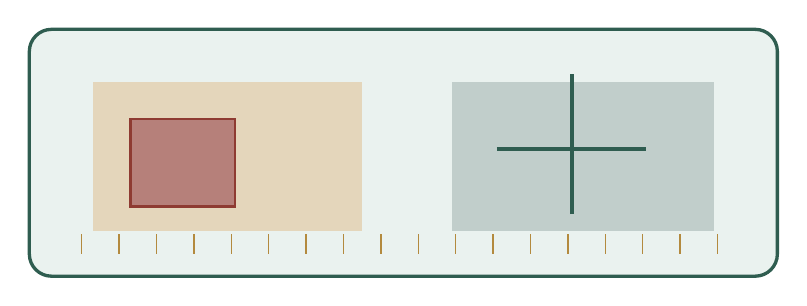
\begin{tikzpicture}[scale=0.95]
		\fill[FarmGreenLight,rounded corners=8pt] (-5,-1.65) rectangle (5,1.65);
		\draw[FarmGreen,line width=1.2pt,rounded corners=8pt] (-5,-1.65) rectangle (5,1.65);
		\fill[FarmGold!35] (-4.15,-1.05) rectangle (-0.55,0.95);
		\fill[FarmGreen!30] (0.65,-1.05) rectangle (4.15,0.95);
		\fill[FarmRed!65] (-3.65,-0.72) rectangle (-2.25,0.45);
		\draw[FarmRed,line width=1pt] (-3.65,-0.72) rectangle (-2.25,0.45);
		\draw[FarmGreen,line width=1.4pt] (2.25,-0.82) -- (2.25,1.05);
		\draw[FarmGreen,line width=1.4pt] (1.25,0.05) -- (3.25,0.05);
		\foreach \x in {-4.3,-3.8,...,4.3} \draw[FarmGold,line width=.5pt] (\x,-1.35)--(\x,-1.08);
	\end{tikzpicture}

	\vspace{0.45cm}
	{\large\bfseries\color{FarmGreen} Interactive 3D Farm Environment\\[0.2cm]}
	{\small\color{Muted} A practical guide to reading, changing, extending, building and testing the project\\[0.75cm]}

	\begin{tcolorbox}[width=0.94\textwidth,colback=white,colframe=CodeBorder,boxrule=0.7pt,arc=2mm,left=4mm,right=4mm,top=3mm,bottom=3mm]
		\noindent\makebox[0.36\linewidth][l]{\bfseries\color{Ink}Repository:}%
		\href{https://github.com/Sivothajan/csc3081_farm_project/tree/de29e8f8a2b92f47097514f5d0ad8c3b512e058d}{\texttt{Sivothajan/csc3081\_farm\_project}}\par\vspace{0.15cm}
		\noindent\makebox[0.36\linewidth][l]{\bfseries\color{Ink}Project author:}%
		Sivothayan .S -- S/21/513\par\vspace{0.15cm}
		\noindent\makebox[0.36\linewidth][l]{\bfseries\color{Ink}Documentation snapshot:}%
		main branch at \code{de29e8f} -- 7 September 2026\par\vspace{0.15cm}
		\noindent\makebox[0.36\linewidth][l]{\bfseries\color{Ink}Full commit:}%
		{\scriptsize\ttfamily de29e8f8a2b92f47097514f5d0ad8c3b512e058d}\par
	\end{tcolorbox}

	\vfill
	{\footnotesize\color{Muted} The repository name above links to the exact commit snapshot documented here.}
\end{titlepage}

\frontmatter
\chapter*{How to use this handbook}
\addcontentsline{toc}{chapter}{How to use this handbook}
This document is designed for a reader who may know only basic C++ and very little OpenGL. You do not need to understand the entire project before changing it. The chapters build a mental model first, then explain each source module, then provide a customization cookbook.

\begin{beginnerbox}
	If you only want to change the appearance, start with \textbf{Part VI: Customization Cookbook}. If you want to understand how the program works, read Parts I--V in order. If a compiler error mentions a file, use the file index in the appendices to jump to that module.
\end{beginnerbox}

The explanations deliberately repeat a few important ideas---especially coordinate axes, RGB colors, OpenGL transforms, the update/render split, and \code{dt}. That repetition is intentional: those concepts appear everywhere in the project and are the keys to editing it confidently.

\section*{What is covered}
\begin{itemize}
	\item Every C++ subsystem under \file{src/}: animals, core, environment, objects, structures, systems, utilities, and vegetation.
	\item Program startup, the FreeGLUT event loop, input, update timing, rendering order, camera movement and projection.
	\item Geometry helpers, vectors, colors, textures, lighting, custom font rendering, the editable text catalog and the HUD.
	\item Wind deformation, grass cutting, crops, trees, cow animation, herd state transitions and barn doors.
	\item CMake, FreeGLUT dependency fetching, Visual Studio project support, build scripts, verification and asset generators.
	\item Concrete recipes for changing positions, dimensions, colors, movement speeds, counts, camera presets, wind behavior, day/night, signs, controls and textures.
	\item How to add a new object, new key binding, new camera view, new texture, and new animated system.
\end{itemize}

\section*{Notation}
\begin{tabularx}{\textwidth}{@{}lX@{}}
	\toprule
	Notation                  & Meaning                                                            \\
	\midrule
	\file{src/core/Scene.cpp} & A repository file path.                                            \\
	\code{CAMERA_SPEED}       & A C++ identifier or literal value.                                 \\
	\keycap{N}                & A keyboard key used by the running application.                    \\
	\rgb{0.66f}{0.23f}{0.17f} & An OpenGL RGB color where each channel is usually between 0 and 1. \\
	\bottomrule
\end{tabularx}

\tableofcontents
\listoftables
\clearpage

\mainmatter
\part{Orientation: Understand the Project Before Editing It}

\chapter{Project Overview}
\section{What Willowfield is}
Willowfield is an interactive 3D farm built using C++20, classic fixed-function OpenGL, GLU and FreeGLUT. The farm contains terrain, dirt and grass areas, paths, fences, a barn, windmill, hay bales, rocks, crops, trees, animated grass, cows, a day/night transition, lighting, textures, signs, a custom handwritten font and a HUD.

The project is intentionally built from relatively small modules. There is no heavy game engine. Instead, each module sends drawing commands to OpenGL. This is excellent for learning because you can follow a visual object from its C++ function directly to the primitives that appear on screen.

\begin{beginnerbox}
	Think of the program as three layers:
	\begin{enumerate}
		\item \textbf{Application loop}: creates the window, reads input and repeatedly asks the scene to update and draw.
		\item \textbf{Scene coordinator}: owns the camera and all farm components, and decides update/render order.
		\item \textbf{Components}: barn, grass, cow, tree, wind, HUD, textures, and so on.
	\end{enumerate}
\end{beginnerbox}

\section{High-level architecture}
\begin{center}
	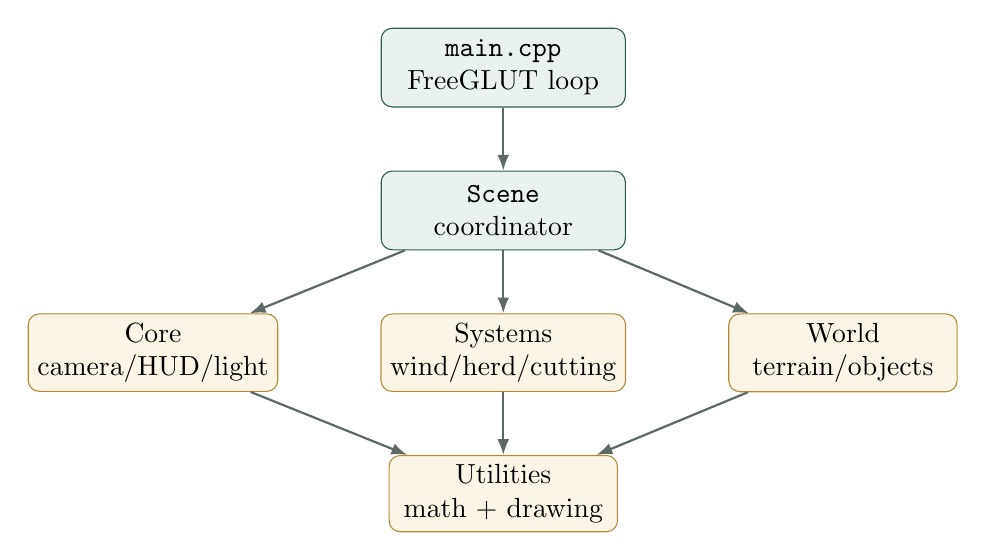
\begin{tikzpicture}[
			node distance=8mm and 13mm,
			box/.style={draw=FarmGreen,rounded corners,fill=FarmGreenLight,align=center,minimum width=31mm,minimum height=10mm},
			sys/.style={draw=FarmGold,rounded corners,fill=FarmGoldLight,align=center,minimum width=29mm,minimum height=9mm},
			arr/.style={-{Latex[length=2mm]},thick,color=Muted}
		]
		\node[box] (main) {\texttt{main.cpp}\\FreeGLUT loop};
		\node[box,below=of main] (scene) {\texttt{Scene}\\coordinator};
		\node[sys,below left=of scene] (core) {Core\\camera/HUD/light};
		\node[sys,below=of scene] (systems) {Systems\\wind/herd/cutting};
		\node[sys,below right=of scene] (world) {World\\terrain/objects};
		\node[sys,below=of systems] (draw) {Utilities\\math + drawing};
		\draw[arr] (main)--(scene);
		\draw[arr] (scene)--(core);
		\draw[arr] (scene)--(systems);
		\draw[arr] (scene)--(world);
		\draw[arr] (core)--(draw);
		\draw[arr] (systems)--(draw);
		\draw[arr] (world)--(draw);
	\end{tikzpicture}
\end{center}

\section{Repository organization}
\begin{longtable}{@{}p{0.31\textwidth}p{0.63\textwidth}@{}}
	\toprule
	Path & Purpose \\
	\midrule
	\endhead
	\pathrow{src/main.cpp}{Application entry point and FreeGLUT callback wiring.}
	\pathrow{src/core/}{Scene coordination, camera, editable text catalog, HUD, lighting, textures, capture and verification.}
	\pathrow{src/environment/}{Terrain, paths and sky/day-night rendering.}
	\pathrow{src/vegetation/}{Grass, crops and trees.}
	\pathrow{src/structures/}{Barn, fences and windmill.}
	\pathrow{src/objects/}{Hay bales, trough and rocks.}
	\pathrow{src/animals/}{Cow model and individual movement/animation logic.}
	\pathrow{src/systems/}{Wind, herd state machine, animation pause/time and grass cutting.}
	\pathrow{src/utils/}{Constants, vector math, drawing primitives and custom font support.}
	\pathrow{assets/}{Runtime textures, generated handwriting atlas, and editable shared labels in \file{assets/text.txt}.}
	\pathrow{cmake/}{FreeGLUT dependency acquisition, embedded text fallback generation, and dependency-only configuration.}
	\pathrow{scripts/}{Build, setup, verification, formatting, project synchronization and asset generation.}
	\pathrow{docs/}{Script instructions, third-party/license notes, and the repository beginner code walkthrough.}
	\pathrow{CMakeLists.txt}{Cross-project CMake definition, linking, post-build asset copy and CTest definitions.}
	\pathrow{csc3081\_farm\_project.vcxproj}{Visual Studio/MSBuild project.}
	\pathrow{csc3081\_farm\_project.slnx}{Visual Studio solution entry point.}
	\bottomrule
\end{longtable}

\section{Main runtime features}
The current controls demonstrate how the modules are connected. Movement uses \keycap{W/A/S/D}; arrow keys or right mouse drag change viewing direction; \keycap{Q/E} changes camera height; \keycap{G} jumps to the meadow; \keycap{H} shows the barn; \keycap{Tab} cycles views; \keycap{N} requests day/night; \keycap{P} pauses animation; \keycap{C} enables grass cutting; \keycap{R} restores grass; \keycap{+/-} changes wind; \keycap{L/T/F} toggle lighting/textures/wireframe; \keycap{B} toggles the structural-study overlay; \keycap{F9} reloads shared labels from \file{assets/text.txt}; and \keycap{F10} hides all overlays.

\chapter{The Three Ideas That Explain Most of the Code}
\section{Update and render are separate}
Interactive graphics programs usually separate \emph{simulation} from \emph{drawing}. Willowfield follows this pattern.

\begin{itemize}
	\item \code{Scene::update(dt)} changes state: wind time advances, the windmill rotates, cows move, the sky transitions, and grass may be cut.
	\item \code{Scene::render(width, height)} reads the current state and draws it. Rendering should not normally decide simulation outcomes.
\end{itemize}

\begin{whybox}
	If movement happened only when an object was rendered, changing frame rate could change simulation behavior. Using \code{dt} (delta time in seconds) makes movement approximately frame-rate independent.
\end{whybox}

\section{OpenGL transformations are local edits to a coordinate system}
The project uses classic OpenGL matrix functions such as \code{glTranslatef}, \code{glRotatef} and \code{glScalef}. The common pattern is:
\begin{lstlisting}[language=C++]
glPushMatrix();
glTranslatef(x, y, z);
glRotatef(angle, 0, 1, 0);
glScalef(sx, sy, sz);
// draw object here
glPopMatrix();
\end{lstlisting}
\code{glPushMatrix()} saves the previous transform, and \code{glPopMatrix()} restores it. Without that pair, moving one object could accidentally move everything drawn afterwards.

\section{Colors are ordinary numbers}
Most material colors are set with \code{glColor3f(r, g, b)} or passed as a \code{Vec3}. Each channel usually ranges from 0 to 1.

\begin{center}
	\begin{tabular}{@{}lll@{}}
		\toprule
		Color idea  & Approximate value                  & Where you see similar values \\
		\midrule
		Dark wood   & \rgb{.42f}{.32f}{.22f}             & Windmill timber              \\
		Barn red    & \rgb{.66f}{.23f}{.17f}             & Barn walls                   \\
		Grass green & \rgb{.32f}{.49f}{.16f}             & Grass blade base color       \\
		Hay gold    & \rgb{.82f}{.64f}{.25f}             & Hay bales                    \\
		Sky blue    & starts near \rgb{.66f}{.81f}{.86f} & Day background               \\
		\bottomrule
	\end{tabular}
\end{center}

\begin{editbox}
	To make an object more red, increase the first number. More green: increase the second. More blue: increase the third. Keep values roughly in the 0--1 range unless you deliberately want clamping.
\end{editbox}

\chapter{The Farm Coordinate System}
\section{What X, Y and Z mean}
Willowfield uses Y as height. The ground is near \code{y = 0}. X moves left/right across the farm and Z moves forward/back across the farm.

\begin{center}
	\begin{tikzpicture}[scale=1.05]
		\coordinate (O) at (0,0);
		\draw[-{Latex},very thick,FarmRed] (O)--(3,0) node[right] {+X};
		\draw[-{Latex},very thick,FarmGreen] (O)--(0,3) node[above] {+Y (up)};
		\draw[-{Latex},very thick,FarmBlue] (O)--(-2,-1.6) node[left] {+Z};
		\node[below right] at (O) {origin (0,0,0)};
	\end{tikzpicture}
\end{center}

\section{Approximate top-down layout}
The following map is reconstructed from the coordinates used by the code. It is not a screenshot; it is a debugging map to help you understand where things are placed.

\begin{center}
	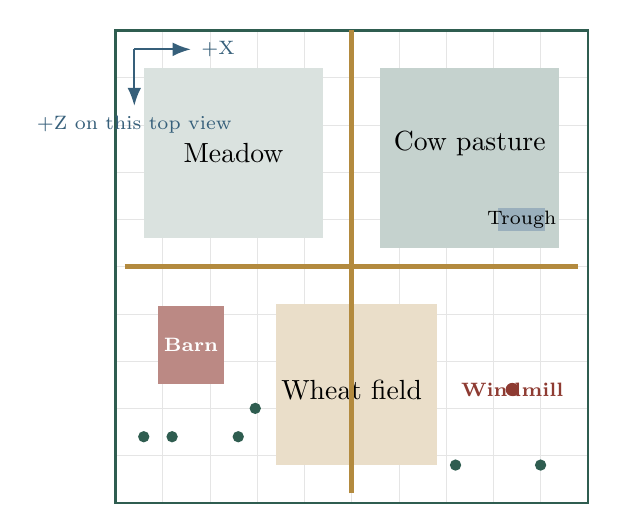
\begin{tikzpicture}[x=0.12cm,y=0.12cm]
		\draw[step=5,very thin,gray!20] (-25,-25) grid (25,25);
		\draw[thick,FarmGreen] (-25,-25) rectangle (25,25);
		\fill[FarmGreen!18] (-22,3) rectangle (-3,21);
		\node at (-12.5,12) {Meadow};
		\fill[FarmGreen!28] (3,2) rectangle (22,21);
		\node at (12.5,13) {Cow pasture};
		\fill[FarmGold!28] (-8,-21) rectangle (9,-4);
		\node at (0,-13) {Wheat field};
		\fill[FarmRed!60] (-20.5,-12.4) rectangle (-13.5,-4.2);
		\node[white,font=\scriptsize\bfseries] at (-17,-8.3) {Barn};
		\fill[FarmBlue!50] (15.5,3.8) rectangle (20.5,6.2);
		\node[font=\scriptsize] at (18,5) {Trough};
		\draw[FarmGold,line width=2pt] (0,-24)--(0,25);
		\draw[FarmGold,line width=2pt] (-24,0)--(24,0);
		\node[FarmRed,font=\scriptsize\bfseries] at (17,-13) {Windmill};
		\fill[FarmRed] (17,-13) circle (0.7);
		\foreach \p in {(-19,-18),(-12,-18),(-22,-18),(-10.2,-15),(11,-21),(20,-21)}
		\fill[FarmGreen] \p circle (0.6);
		\draw[-{Latex},thick,FarmBlue] (-23,23)--(-17,23) node[right,font=\scriptsize] {+X};
		\draw[-{Latex},thick,FarmBlue] (-23,23)--(-23,17) node[below,font=\scriptsize] {+Z on this top view};
	\end{tikzpicture}
\end{center}

\begin{warningbox}
	Changing an object's position may also require changing related routes or camera presets. For example, moving the barn without changing \code{Barn::aisle()}, \code{Barn::bed()}, herd routes and barn camera targets would make cows walk to the old barn location.
\end{warningbox}

\part{Program Core: Startup, Timing, Input and Scene Coordination}

\chapter{\texttt{src/main.cpp}: The Application Entry Point}
\section{Responsibility}
\file{src/main.cpp} is the glue between FreeGLUT and the rest of the application. It owns one global \code{Scene}, keyboard-state arrays, window dimensions, frame counters and callback state. It does not draw individual barns or cows itself; it delegates that work to \code{Scene}.

\section{Important global state}
\begin{tabularx}{\textwidth}{@{}lX@{}}
	\toprule
	Variable             & Meaning                                                                        \\
	\midrule
	\code{Scene scene}   & The complete farm world.                                                       \\
	\code{keys[256]}     & Whether ordinary keyboard keys are currently held.                             \\
	\code{special[256]}  & Whether FreeGLUT special keys, such as arrows/F-keys, are held.                \\
	\code{width, height} & Current window dimensions; defaults are 1280 by 800.                           \\
	\code{previousTime}  & Used to calculate frame delta time.                                            \\
	\code{closing}       & Prevents callbacks from touching a window/context while it is being destroyed. \\
	\code{capturePath}   & Enables deterministic frame capture for verification.                          \\
	\bottomrule
\end{tabularx}

\section{Frame callback: \texttt{display()}}
The display callback performs one rendered frame:
\begin{enumerate}
	\item Stop immediately if the window is closing.
	\item Ask the scene for the background clear color.
	\item Clear color and depth buffers.
	\item Reset the model-view matrix.
	\item Apply the camera transform.
	\item Render the scene.
	\item Optionally capture the third frame for automated verification.
	\item Swap front/back buffers.
	\item Optionally finish a benchmark.
\end{enumerate}

\begin{lstlisting}[language=C++]
scene.background();
glClear(GL_COLOR_BUFFER_BIT | GL_DEPTH_BUFFER_BIT);
glMatrixMode(GL_MODELVIEW);
glLoadIdentity();
scene.camera.apply();
scene.render(width, height);
glutSwapBuffers();
\end{lstlisting}

\begin{beginnerbox}
	Double buffering means the next frame is drawn into a hidden back buffer. \code{glutSwapBuffers()} then displays it all at once. This avoids visible partial drawing and flicker.
\end{beginnerbox}

\section{Projection callback: \texttt{reshape()}}
When the window changes size, \code{reshape()} updates the viewport and perspective projection.
\begin{lstlisting}[language=C++]
gluPerspective(55, double(width) / height, 0.08, 160);
\end{lstlisting}
The four parameters are field of view, aspect ratio, near clipping distance and far clipping distance.

\begin{editbox}
	Want a wider-angle view? Increase \code{55}. Want a more zoomed-in lens? Decrease it. Extreme values can cause distortion. The near plane \code{0.08} should stay positive.
\end{editbox}

\section{Update callback: \texttt{update()}}
The timer callback calculates \code{dt}, updates the camera, updates the scene, requests a redraw and schedules the next timer roughly 16 ms later.
\begin{lstlisting}[language=C++]
float dt = std::clamp(float(now - previousTime) / 1000.0f, 0.0f, 0.05f);
scene.camera.update(dt, keys, special);
scene.update(dt);
glutPostRedisplay();
glutTimerFunc(16, update, 0);
\end{lstlisting}
The upper clamp of 0.05 seconds prevents an enormous simulation jump after a pause or hitch.

\section{Input callbacks}
Ordinary key presses call \code{scene.key(lower)} only on the transition from not-held to held. This is why toggle keys do not rapidly switch every update while you hold them. Continuous movement is handled by the held-key arrays in \code{Camera::update()}.

Right-mouse drag converts mouse pixel differences to yaw/pitch changes at \code{0.2f} degrees per pixel.

\section{Program startup}
\code{main()} parses test/capture options, initializes FreeGLUT, asks for double-buffered RGB + depth + multisampling, creates the window, enables depth testing and normal normalization, initializes the scene, registers callbacks and enters \code{glutMainLoop()}.

\begin{warningbox}
	The code intentionally gives FreeGLUT only the program name through a local \code{glutArgc = 1}. Application-specific switches are parsed first so GLUT does not try to interpret them.
\end{warningbox}

\chapter{\texttt{Scene}: The Central Coordinator}
\section{Files}
\begin{filebox}{src/core/Scene.h}
	Defines the \code{Scene} class. It owns every major subsystem and exposes \code{initialize}, \code{update}, \code{render}, \code{key} and \code{specialKey}.
\end{filebox}
\begin{filebox}{src/core/Scene.cpp}
	Implements initialization, frame updates, key bindings and the exact render order.
\end{filebox}

\section{What the Scene owns}
The scene owns a camera plus terrain, path, fence, windmill, barn, rocks, hay, lighting, wind, grass, crops, trees, herd, animation state, cutting system, HUD, textures and sky. It also stores a short-lived text-reload notice. The shared text catalog itself is global through the \code{Text} namespace. This means \code{Scene} remains the natural place to add a new top-level farm component.

\begin{lstlisting}[language=C++]
Terrain terrain;
Path path;
Fence fence;
Windmill windmill;
Barn barn;
Rock rocks;
HayBale hay;
Lighting lighting;
WindSystem wind;
Grass grass;
Crop crops;
Tree trees;
Herd herd;
AnimationSystem animation;
GrassCuttingSystem cutting;
Hud hud;
float textNoticeTime = 0;
std::string textNotice;
TextureSet textures;
Sky sky;
\end{lstlisting}

\section{Initialization}
Only modules that need startup work are explicitly initialized:
\begin{lstlisting}[language=C++]
Text::initialize(executable);
grass.initialize();
crops.initialize();
textures.initialize(executable);
Font::initialize(executable);
\end{lstlisting}
\code{Text::initialize()} first resolves the editable \file{assets/text.txt}; grass and crops then generate deterministic procedural layouts. Textures and the font atlas locate runtime assets relative to the executable, with a fallback to a local \file{assets} directory.

\section{Update order}
\begin{center}
	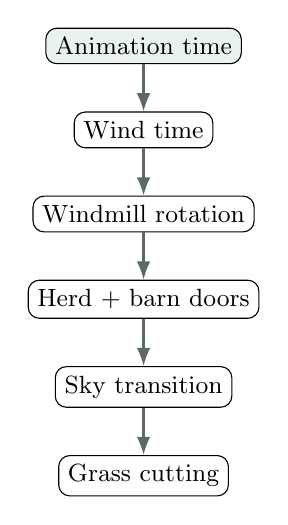
\begin{tikzpicture}[node distance=6mm, every node/.style={font=\small}, arr/.style={-{Latex},thick,Muted}]
		\node[draw,rounded corners,fill=FarmGreenLight] (anim) {Animation time};
		\node[draw,rounded corners,below=of anim] (wind) {Wind time};
		\node[draw,rounded corners,below=of wind] (mill) {Windmill rotation};
		\node[draw,rounded corners,below=of mill] (herd) {Herd + barn doors};
		\node[draw,rounded corners,below=of herd] (sky) {Sky transition};
		\node[draw,rounded corners,below=of sky] (cut) {Grass cutting};
		\draw[arr] (anim)--(wind); \draw[arr] (wind)--(mill); \draw[arr] (mill)--(herd); \draw[arr] (herd)--(sky); \draw[arr] (sky)--(cut);
	\end{tikzpicture}
\end{center}
Before animated systems advance, \code{textNoticeTime} is reduced so the F9 success/failure message disappears after five seconds. \code{AnimationSystem::update()} returns zero while paused, so downstream animated systems stop naturally.

\section{Keyboard commands}
\begin{longtable}{@{}lll@{}}
	\toprule
	Key             & Scene action                  & Module affected    \\
	\midrule
	\endhead
	\keycap{V}      & Overview preset               & Camera             \\
	\keycap{G}      & Meadow camera                 & Camera             \\
	\keycap{H}      & Barn camera                   & Camera             \\
	\keycap{Tab}    & Next preset                   & Camera             \\
	\keycap{+/=}    & Wind +0.25                    & WindSystem         \\
	\keycap{-}      & Wind -0.25                    & WindSystem         \\
	\keycap{0..3}   & Exact wind preset             & WindSystem         \\
	\keycap{C}      & Toggle cutting                & GrassCuttingSystem \\
	\keycap{R}      & Restore grass                 & Grass              \\
	\keycap{P}      & Pause/resume                  & AnimationSystem    \\
	\keycap{B}      & Toggle structural study       & HUD state          \\
	\keycap{L}      & Lighting on/off               & Lighting           \\
	\keycap{F}      & Wireframe on/off              & Renderer           \\
	\keycap{T}      & Textures on/off               & TextureSet usage   \\
	\keycap{N}      & Toggle requested night        & Sky/Herd           \\
	\keycap{F1..F8} & Camera preset                 & Camera             \\
	\keycap{F9}     & Reload \file{assets/text.txt} & Text/HUD notice    \\
	\keycap{F10}    & HUD on/off                    & Hud                \\
	\bottomrule
\end{longtable}

\section{Render order matters}
The render function applies lighting and barn light, selects wireframe/fill mode, then draws sky, terrain, path, fence, windmill, barn, rocks, hay, vegetation, herd, cutting indicator and finally HUD.

\begin{beginnerbox}
	Later drawing can depend on earlier OpenGL state. The code deliberately binds/turns off textures between groups. When adding a component, decide whether it needs textures, lighting, blending or wireframe and avoid leaking state into later components.
\end{beginnerbox}

\chapter{Camera System}
\section{Files and data}
\file{src/core/Camera.h} defines eight named views plus the current position, yaw and pitch. The initial overview is:
\begin{lstlisting}[language=C++]
Vec3 position{33, 27, 37};
float yaw = -132.0f, pitch = -29.5f;
\end{lstlisting}

\section{Continuous movement}
Yaw determines the horizontal forward direction. The camera creates forward/right vectors and combines held WASD keys. Q/E modifies Y. If the movement vector is nonzero, it is normalized before multiplying by camera speed and \code{dt}.

\begin{lstlisting}[language=C++]
Vec3 forward{std::cos(y), 0, std::sin(y)};
Vec3 right{-std::sin(y), 0, std::cos(y)};
Vec3 move = forward * (float(keys['w']) - float(keys['s'])) +
            right * (float(keys['d']) - float(keys['a']));
move.y = float(keys['e']) - float(keys['q']);
position = position + normalized(move) * (Constants::CAMERA_SPEED * dt);
\end{lstlisting}

\section{Bounds}
The camera is clamped to:
\begin{itemize}
	\item X: -34 to +34
	\item Z: -34 to +38
	\item Y: \code{Constants::EYE_MIN} (1.35) to 30
	\item Pitch: -80 to +80 degrees
\end{itemize}
These limits protect the user from going under the ground or beyond useful viewing space.

\section{Localized view names}
The coordinates of the eight presets are still hardcoded in \file{Camera.cpp}, but their displayed names are now data-driven. \code{customName} stores a text key such as \code{"view.free"} or \code{"view.meadow"}, and \code{viewName()} resolves keys through \code{Text::get()}.

\begin{lstlisting}[language=C++]
const std::string& Camera::viewName() const {
    if (customName)
        return Text::get(customName);
    const char* names[]{"view.overview", "view.front", "view.back", "view.left",
                        "view.right", "view.barn", "view.barn_left", "view.barn_right"};
    return Text::get(names[static_cast<int>(selected)]);
}
\end{lstlisting}

\begin{editbox}
	To rename a camera view, edit the matching \code{view.*} value in \file{assets/text.txt} and press \keycap{F9}. Do not change the key in \file{Camera.cpp} unless you intentionally change the text-catalog API.
\end{editbox}

\section{Preset views}
\begin{longtable}{@{}llll@{}}
	\toprule
	View       & Position                    & Target idea      & Shortcut \\
	\midrule
	\endhead
	Overview   & \code{\{33,27,37\}}         & Farm origin      & F1       \\
	Front      & \code{\{0,23,38\}}          & Farm center      & F2       \\
	Back       & \code{\{0,23,-34\}}         & Near center      & F3       \\
	Left       & \code{\{-34,23,2\}}         & Across farm      & F4       \\
	Right      & \code{\{34,23,2\}}          & Across farm      & F5       \\
	Barn       & \code{Barn::viewPosition()} & Barn interior    & F6 / H   \\
	Barn left  & \code{\{-19.8,3.1,-5.0\}}   & Left stall side  & F7       \\
	Barn right & \code{\{-14.2,3.1,-5.0\}}   & Right stall side & F8       \\
	\bottomrule
\end{longtable}

\begin{editbox}
	To create a more cinematic overview, edit only the Overview position/target in \file{src/core/Camera.cpp}. To change free-walk speed, edit \code{CAMERA_SPEED} in \file{src/utils/Constants.h}. Keep the position inside the clamp bounds or your preset will be corrected as soon as movement updates.
\end{editbox}

\chapter{Constants and Vector Math}
\section{\texttt{src/utils/Constants.h}}
This small file remains one of the best places for a beginner to start customizing numeric behavior. Author/title metadata no longer lives here; it moved to \file{assets/text.txt}.
\begin{lstlisting}[language=C++]
constexpr float CAMERA_SPEED = 6.0f;
constexpr float EYE_MIN = 1.35f;
constexpr float WIND_MAX = 3.0f;
constexpr float CUT_RADIUS = 1.8f;
constexpr int GRASS_SEGMENTS = 5;
\end{lstlisting}

\begin{longtable}{@{}p{0.22\textwidth}p{0.14\textwidth}p{0.56\textwidth}@{}}
	\toprule
	Constant              & Current & Effect                                                                                          \\
	\midrule
	\endhead
	\code{CAMERA_SPEED}   & 6.0     & Units per second for normalized free-camera movement.                                           \\
	\code{EYE_MIN}        & 1.35    & Lowest allowed camera height.                                                                   \\
	\code{WIND_MAX}       & 3.0     & Upper clamp for wind strength.                                                                  \\
	\code{CUT_RADIUS}     & 1.8     & Horizontal grass-cutting radius around camera.                                                  \\
	\code{GRASS_SEGMENTS} & 5       & Number of deformable sections in each grass blade. Higher is smoother but draws more triangles. \\
	\bottomrule
\end{longtable}

\section{\texttt{src/utils/MathUtils.h}}
\code{Vec3} is a tiny three-float vector type. It supports addition, subtraction and scaling. Utility functions provide degrees-to-radians conversion, length, normalization, cross product and 2D squared distance.

\begin{lstlisting}[language=C++]
struct Vec3 {
    float x = 0, y = 0, z = 0;
    Vec3 operator+(Vec3 b) const { return {x + b.x, y + b.y, z + b.z}; }
    Vec3 operator-(Vec3 b) const { return {x - b.x, y - b.y, z - b.z}; }
    Vec3 operator*(float s) const { return {x * s, y * s, z * s}; }
};
\end{lstlisting}

\begin{beginnerbox}
	\code{distanceSquared2D()} ignores height and avoids a square root. That is ideal for grass cutting: the system only cares whether the player's X/Z location is inside a circular radius on the ground.
\end{beginnerbox}

\chapter{Drawing Helpers: Boxes, Ellipsoids, Beams, Ground and Signs}
\section{Files}
\file{src/utils/Helpers.h} declares drawing utilities in namespace \code{Draw}. \file{Helpers.cpp} implements them with immediate-mode OpenGL and FreeGLUT primitives.

\section{\texttt{Draw::box}}
Boxes are drawn explicitly as six quads with normals and UV coordinates. This is more work than a GLUT cube, but it supports texture coordinates on every face.

\begin{lstlisting}[language=C++]
void box(Vec3 center, Vec3 size, Vec3 color);
\end{lstlisting}
Interpret the arguments as:
\begin{itemize}
	\item \code{center}: object location.
	\item \code{size}: total width/height/depth along X/Y/Z.
	\item \code{color}: fallback/material color.
\end{itemize}

\section{\texttt{Draw::ellipsoid}}
This scales a unit sphere. For example, \code{\{1.15,.63,.58\}} creates the elongated cow torso.

\section{\texttt{Draw::beam}}
A beam is a cylinder aligned from point A to point B. The function computes the direction and rotates FreeGLUT's +Z cylinder into that direction. It is reused for fence rails, tree branches, horns, straw, roof/detail pieces and more.

\section{\texttt{Draw::ground}}
Ground is one horizontal textured quad with a normal and repeated UV coordinates. The \code{repeat} parameter controls how many texture repetitions span the rectangle.

\section{\texttt{Draw::triangle}}
The helper computes a surface normal from the cross product of two triangle edges, then sends the three vertices. Vegetation uses this heavily.

\section{Signs and plaques}
\code{Draw::plaque()} reads the current model-view matrix and rotates the board around Y so its face follows the camera. It draws a wooden board, a darker face panel and custom text. \code{Draw::sign()} adds a vertical post and places a plaque above it.

\begin{editbox}
	To change every sign's standard size, edit \code{Draw::sign()} in \file{Helpers.cpp}. The current plaque is about 3.2 units wide and 1 unit tall. To change only one sign's wording or position, edit the call in \file{Path.cpp}.
\end{editbox}

\part{Rendering Infrastructure: Light, Texture, Font and HUD}

\chapter{Lighting}
\section{Global light}
\file{src/core/Lighting.cpp} enables fixed-function lighting when requested. It configures two-sided lighting, color material, a global ambient term and a directional light (\code{GL\_LIGHT0}). Day/night modifies ambient and diffuse intensities using the continuously varying night amount.

\begin{lstlisting}[language=C++]
const GLfloat direction[] = {-0.5f, 1.0f, 0.6f, 0};
\end{lstlisting}
The fourth value 0 means this is a directional light rather than a point light.

\section{Barn night light}
\code{Barn::light()} uses \code{GL\_LIGHT1} as a warm point light near \code{\{-17, 3.3, -8.5\}}. Its brightness scales with \code{nightAmount}, and attenuation makes it weaken with distance.

\begin{editbox}
	For a warmer barn lamp, increase red relative to green/blue in the diffuse array. For a larger effective radius, reduce linear/quadratic attenuation values. Large reductions can make the light unrealistically strong across the whole farm.
\end{editbox}

\chapter{Textures and BMP Loading}
\section{Surface categories}
\file{src/core/Texture.h} defines four surfaces:
\begin{lstlisting}[language=C++]
enum class Surface { Ground, Dirt, Wood, Hay, Count };
\end{lstlisting}
The corresponding BMP files are:
\begin{itemize}
	\item \file{assets/textures/terrain/grass\_ground.bmp}
	\item \file{assets/textures/terrain/dirt.bmp}
	\item \file{assets/textures/structures/wood.bmp}
	\item \file{assets/textures/structures/hay.bmp}
\end{itemize}

\section{How the loader works}
\code{TextureSet::loadBmp()} manually validates a simple 24-bit uncompressed BMP, reads padded rows, converts BGR file order into RGB, creates an OpenGL texture and builds mipmaps. It accepts dimensions up to 4096 in either direction.

\begin{warningbox}
	The runtime loader expects 24-bit uncompressed BMP. If you replace a texture with a PNG or compressed BMP without also changing the loader, it will fail and the project will fall back to material colors.
\end{warningbox}

\section{Fallback behavior}
Missing textures are not fatal. Initialization prints a warning and leaves the texture ID at zero. \code{bind()} disables texturing when the requested texture is missing. This is why verification includes a no-assets startup test.

\section{Texture generation}
\file{scripts/generate-textures.py} procedurally creates the four 64x64 24-bit BMP textures with fixed random seeds 3081--3084. No third-party images or Python packages are needed.

\chapter{Custom Font and World-Space Labels}
\section{Files}
\file{src/utils/Font.cpp} loads \file{assets/fonts/handwriting.bmp}. \file{FontMetrics.h} stores generated glyph advance widths for printable ASCII. If the atlas is missing, the renderer falls back to FreeGLUT Roman stroke characters.

\section{Atlas layout}
The atlas is generated by \file{scripts/generate-font.py} from Patrick Hand. It uses 64x80 cells in a 1024x512 bitmap and generates measurements for ASCII characters 32--126.

\section{Regenerating}
The documented maintenance flow creates a Python environment, installs Pillow 12.1.1 and runs the generator. The source font is checksum-verified before use.

\begin{editbox}
	Changing the font requires regenerating both the bitmap atlas and \file{FontMetrics.h}; replacing only the bitmap may make spacing incorrect. The runtime itself does not require Pillow or the original TTF.
\end{editbox}


\chapter{Editable Text Catalog: \texttt{assets/text.txt} and \texttt{Text.*}}
\section{Why this system was added}
User-facing wording is no longer scattered across \file{Hud.cpp}, \file{Camera.cpp}, \file{Path.cpp}, \file{Barn.cpp}, \file{Herd.cpp} and \file{Cow.cpp}. The repository now has one plain-text catalog at \file{assets/text.txt}. A beginner can rename the farm, signs, stalls, views and status messages without recompiling C++.

\begin{filebox}{assets/text.txt}
	The editable source of user-facing labels. Each meaningful line is \code{key = value}. Lines starting with \code{\#} and blank lines are ignored.
\end{filebox}
\begin{filebox}{src/core/Text.h / src/core/Text.cpp}
	Defines \code{TextCatalog}, runtime loading/reloading, key lookup and placeholder formatting.
\end{filebox}
\begin{filebox}{cmake/EmbedText.cmake / cmake/TextDefaults.h.in}
	Embeds the same text file into a generated header at configure time so missing files or omitted keys still have built-in defaults.
\end{filebox}

\section{Important text groups}
\begin{longtable}{@{}p{0.27\textwidth}p{0.63\textwidth}@{}}
	\toprule
	Keys                                     & What they control                                                       \\
	\midrule
	\endhead
	\code{farm.title}, \code{farm.author}    & HUD title and author/course line.                                       \\
	\code{view.*}                            & Camera-view names and the combined view/day/sleep status line.          \\
	\code{herd.*}                            & Grazing, gathering, entering, sleeping, leaving and returning messages. \\
	\code{wind.*}                            & Wind title, controls and still/breeze descriptions.                     \\
	\code{study.*}                           & Structural-study title, hidden-state hint, root/tip labels and formula. \\
	\code{help.*}                            & Bottom control-overlay lines.                                           \\
	\code{cutting.*}                         & Cutting on/off/status and high-camera guidance.                         \\
	\code{text.reloaded}, \code{text.failed} & Temporary F9 feedback.                                                  \\
	\code{sign.*}                            & Meadow, pasture and wheat-field signs.                                  \\
	\code{stall.1..3}                        & Barn stall plaques.                                                     \\
	\code{sleep.symbol}                      & Characters drawn above a sleeping cow.                                  \\
	\bottomrule
\end{longtable}

\section{Live reload with F9}
\code{Scene::specialKey()} handles \keycap{F9}. It calls \code{Text::reload()}, stores either \code{text.reloaded} or \code{text.failed}, and displays that notice for five seconds in the bottom overlay. This means normal label edits do not require a rebuild.

\begin{lstlisting}[language=C++]
if (key == GLUT_KEY_F9) {
    bool loaded = Text::reload();
    textNotice = Text::get(loaded ? "text.reloaded" : "text.failed");
    textNoticeTime = 5;
}
\end{lstlisting}

\section{Parsing and safety rules}
The loader starts from the embedded defaults, then overlays values from the external file. It trims spaces, accepts an optional UTF-8 BOM on the first line, ignores blank/comment lines, and rejects malformed entries. A line must contain \code{=}; both key and value must be nonempty; the line must be at most 1024 characters; and values must contain printable ASCII characters only (codes 32--126).

If loading fails, \code{TextCatalog::load()} leaves the current catalog unchanged. This is why a malformed live edit shows the failure message while the previous labels remain visible.

\begin{warningbox}
	The file comments say to keep keys and \code{\{placeholders\}} unchanged. That is important. Code asks for exact keys such as \code{view.front}. Format strings also rely on placeholder names such as \code{\{view\}}, \code{\{period\}}, \code{\{count\}}, \code{\{value\}}, \code{\{maximum\}} and \code{\{mode\}}.
\end{warningbox}

\section{Placeholder formatting}
\code{Text::format()} scans a catalog value for braces and substitutes supplied name/value pairs. For example, \code{view.status = \{view\} / \{period\} / \{count\} asleep} is filled by the HUD at runtime.

\section{Where the file is loaded from}
At startup the code first looks for \file{assets/text.txt} relative to the current working directory. If it is not there, it tries the \file{assets/text.txt} beside the executable. This is convenient in development and after copying a built application.

\section{Embedded fallback at build time}
\file{cmake/EmbedText.cmake} reads \file{assets/text.txt} during CMake configuration and produces \file{generated/TextDefaults.h} from \file{cmake/TextDefaults.h.in}. The main target and dependency-only build both add the generated directory to include paths. The generated header is a fallback; \file{assets/text.txt} remains the file you should edit.

\begin{editbox}
	For almost every wording change, edit only the value after \code{=} in \file{assets/text.txt}, save, then press \keycap{F9}. Examples: change \code{farm.title}, rename \code{stall.1}, rewrite \code{sign.meadow}, or shorten \code{help.views}. No C++ edit is required.
\end{editbox}

\chapter{HUD: On-Screen Information and Controls}
\section{State passed to the HUD}
\code{HudState} contains cutting status, pause status, whether the structural study is shown, cut-blade count, camera height, herd-status text, sleeping-cow count, day/night, camera-view name and an optional text-reload notice.

\section{Rendering mode}
The HUD temporarily disables depth testing, lighting, textures and fog, enables alpha blending, switches to an orthographic projection, draws panels/text, then restores previous OpenGL state. It does \emph{not} shrink the 3D viewport; the farm continues to fill the whole window behind the overlays.

\section{Current compact layout}
The latest HUD uses the same overlay concept in every camera view instead of a separate ``focused-view'' layout:
\begin{itemize}
	\item top-left: farm title, author line, localized view/day/asleep status, herd or pause status;
	\item top-right: wind value, 12-bar meter, controls and wind description;
	\item bottom: movement/actions/view-help and cutting/reload status;
	\item right above the bottom controls: structural-study panel, or a short \keycap{B} hint when hidden.
\end{itemize}

The overlay scales down when the window is smaller than roughly 960x640. Internally, \code{scale} is the minimum of 1, \code{width/960}, and \code{height/640}; drawing coordinates are then expressed in a stable virtual space. The bottom controls switch between one/two-line arrangements using a \code{wide} check near virtual width 1000.

\section{Text is data-driven}
Nearly all visible wording comes through \code{Text::get()} or \code{Text::format()}. This includes title, author, view status, herd status, wind labels, help, cutting state and study labels. Edit \file{assets/text.txt} rather than hardcoding new strings in \file{Hud.cpp}.

\section{Things you can safely tune}
\begin{longtable}{@{}p{0.32\textwidth}p{0.58\textwidth}@{}}
	\toprule
	Goal                     & Where                                                                                        \\
	\midrule
	\endhead
	Panel background         & \code{panel()} in \file{src/core/Hud.cpp}; currently \rgb{.075f}{.14f}{.13f} with alpha .82. \\
	All user-facing wording  & \file{assets/text.txt}; save and press \keycap{F9}.                                          \\
	Top-left panel size      & \code{leftWidth} and the \code{126} panel height.                                            \\
	Wind panel position/size & \code{studyX}, width 268 and height 104.                                                     \\
	Wind bar geometry        & 12 bars, 20-unit spacing, 15x8 rectangles.                                                   \\
	Study panel height       & 136 units while visible, 36 while hidden.                                                    \\
	Study curve detail       & Loop samples 0..10 and \code{graphScale = 64}.                                               \\
	Small-window scaling     & Denominators 960 and 640 in the \code{scale} calculation.                                    \\
	\bottomrule
\end{longtable}

\begin{warningbox}
	The HUD is deliberately edge-anchored and tested at small window sizes. If you enlarge panels or text substantially, verify 640x480 captures so the top-left and top-right panels do not collide.
\end{warningbox}

\chapter{Terrain}
\section{Files}
\file{src/environment/Terrain.h} declares one \code{render()} method. \file{Terrain.cpp} draws the ground foundation, the overall farm surface, meadow/pasture color regions, dirt field and raised crop furrows.

\section{Main geometry}
\begin{longtable}{@{}p{0.25\textwidth}p{0.31\textwidth}p{0.36\textwidth}@{}}
	\toprule
	Element      & Coordinates                                           & Meaning                                    \\
	\midrule
	\endhead
	Base slab    & center \code{\{0,-.7,0\}}, size \code{\{50,1.35,50\}} & Thick brown ground volume beneath surface. \\
	Farm surface & X/Z -25 to +25                                        & Main 50x50 ground area.                    \\
	Meadow       & X -22..-3, Z 3..21                                    & Darker grass region.                       \\
	Pasture      & X 3..22, Z 2..21                                      & Lighter grass region.                      \\
	Crop dirt    & X -8..9, Z -21..-4                                    & Wheat field base.                          \\
	Furrows      & every 1.15 along X                                    & Raised narrow dirt strips.                 \\
	\bottomrule
\end{longtable}

\begin{editbox}
	To make the whole farm larger, changing only the main 50x50 ground is not enough. You would also need to adjust the perimeter fence, camera bounds, object placements and probably overview camera. For a beginner, resize individual zones instead of the entire world first.
\end{editbox}

\chapter{Paths and Signs}
\file{src/environment/Path.cpp} draws three dirt path rectangles and three signs.

\begin{lstlisting}[language=C++]
Draw::sign({-3, 0, 21}, Text::get("sign.meadow"), Text::get("sign.meadow_hint"));
Draw::sign({4, 0, 19}, Text::get("sign.pasture"));
Draw::sign({-4, 0, -3}, Text::get("sign.wheat"));
\end{lstlisting}

The main paths cross at the world center: a north-south path approximately 3.6 units wide and an east-west path also approximately 3.6 units wide. A branch runs toward the windmill area.

\begin{editbox}
	Renaming a zone is now even safer: edit the matching \code{sign.*} value in \file{assets/text.txt} and press \keycap{F9}. Moving the physical sign is still a C++ edit: change only the first position vector in \file{Path.cpp}.
\end{editbox}

\chapter{Sky and Day/Night Transition}
\section{State}
\code{Sky} contains a boolean target \code{night} and a float \code{nightAmount}. The boolean says where the transition should go; the float says how far the transition has progressed.

\section{Transition speed}
\begin{lstlisting}[language=C++]
float change = dt * .4f;
nightAmount = std::clamp(nightAmount + (night ? change : -change), 0.0f, 1.0f);
\end{lstlisting}
At 0.4 per second, a full transition takes roughly 2.5 seconds.

\section{Background interpolation}
The clear color starts near a bright blue and subtracts channel-specific amounts as night increases. This creates a darker, bluer night background.

\section{Clouds and celestial body}
Five groups of ellipsoids create clouds. Their X position drifts slowly using \code{time * .25f}. A sphere near \code{\{-27,25,-35\}} acts as a bright sun/moon-like object with color changing as night increases.

\begin{editbox}
	To slow the day/night fade, reduce \code{.4f}. To slow cloud movement, reduce \code{.25f}. To add more cloud groups, increase the outer loop count, but remember that each group draws four ellipsoids.
\end{editbox}

\chapter{Wind System: The Shared Deformation Engine}
\section{State}
\file{src/systems/WindSystem.h} starts with strength 1.2, time 0 and wave speed 2.2. The fixed wind direction is approximately \code{\{0.8944,0,0.4472\}}, meaning mostly +X with some +Z.

\section{Displacement formula}
The implementation combines a slow gust wave, a main wave, a secondary wave and the crucial height term \(u^2\):
\[
	D = \text{strength}\times\text{gust}\times\text{wave}\times u^2
\]
Here \(u=0\) at the root and \(u=1\) at the tip.

\begin{center}
	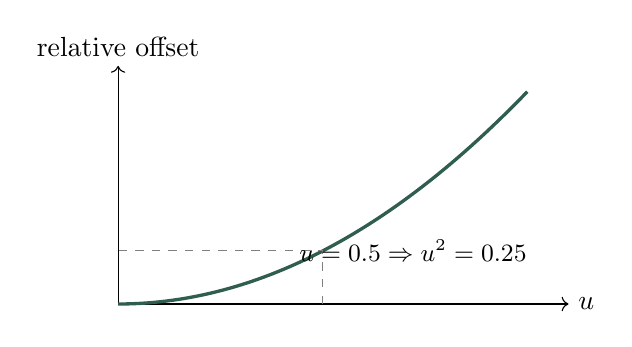
\begin{tikzpicture}[x=5.2cm,y=2.7cm]
		\draw[->] (0,0)--(1.1,0) node[right] {$u$};
		\draw[->] (0,0)--(0,1.12) node[above] {relative offset};
		\draw[FarmGreen,very thick,domain=0:1,samples=60] plot (\x,{\x*\x});
		\draw[dashed,gray] (.5,0)--(.5,.25)--(0,.25);
		\node[font=\small,align=left] at (.72,.25) {$u=0.5\Rightarrow u^2=0.25$};
	\end{tikzpicture}
\end{center}

\begin{beginnerbox}
	The square is why the roots stay visually anchored. At quarter height, the displacement is only \(1/16\) of the tip displacement. This behavior is explicitly tested by the verification suite.
\end{beginnerbox}

\section{\texttt{bend()}}
\code{bend()} returns the original vertical point plus wind-direction offset. Parameters let grass, crops and trees use different flexibility/frequency values while sharing the same wind field.

\begin{editbox}
	Change \code{speed = 2.2f} for faster/slower oscillation. Change the returned direction vector to rotate prevailing wind. Change the \code{.32f} factor in \code{bend()} to scale visible bending globally. Make one plant type react differently by changing its flexibility argument instead of the global formula.
\end{editbox}

\chapter{Grass: Procedural Blades and Cutting}
\section{Initialization}
\file{src/vegetation/Grass.cpp} uses a fixed Mersenne Twister seed 3081. Exactly 2800 blades are generated: the first 2300 belong to the meadow and are cuttable; the remaining 500 are decorative grass elsewhere and not cuttable.

\begin{lstlisting}[language=C++]
for (int i = 0; i < 2800; ++i) {
    const bool meadow = i < 2300;
    // choose x, z, height, width, orientation, phase and response
}
\end{lstlisting}

\section{Meadow range}
Meadow blades use roughly:
\begin{itemize}
	\item X: -21.5 plus up to 18 units
	\item Z: 3.3 plus up to 17 units
	\item Height: 0.55 to 1.15 units
	\item Width: 0.10 to 0.165 units
	\item Wind response: about 0.8 to 1.2
\end{itemize}

\section{Rendering}
Each blade is divided into \code{GRASS_SEGMENTS} sections. For each segment, the code finds two deformed centerline points, narrows the width toward the tip, assigns a slightly varying green tone and draws two triangles.

With 2800 blades and 5 segments, that is roughly \(2800\times5\times2=28{,}000\) grass triangles per frame.

\section{Cutting}
\code{cutNear()} scans blades and checks 2D squared distance. A newly cut blade changes to 22\% of its original height and records \code{cut=true}. A second pass does not shrink it again. \code{reset()} restores every original height.

\begin{editbox}
	Common grass edits:
	\begin{itemize}
		\item Denser field: increase 2800 and/or 2300, at a rendering cost.
		\item Taller meadow: increase \code{.55f} and/or the \code{.60f} random range.
		\item Different green: edit \code{glColor3f(.32f + ..., .49f + ..., .16f + ...)}.
		\item Shorter cut result: reduce \code{.22f}.
		\item Wider cutting area: change \code{CUT_RADIUS} in \file{Constants.h}.
	\end{itemize}
\end{editbox}

\chapter{Crops: Wheat Rows}
\section{Layout}
Crops are generated in regular X rows from about -7.3 to 9 with 1.15 spacing, matching the terrain furrows. Rows close to the central path (\(|x|<2.2\)) are skipped. Z positions run from about -20.2 to -4.4 with 0.42 spacing.

Each stalk height is approximately 1.3 to 1.8 units.

\section{Rendering shape}
A stalk uses two crossed ribbon axes so it has visible width from multiple viewing directions. Leaves and seed heads are attached to the same wind-deformed centerline.

\section{Key visual colors}
\begin{itemize}
	\item Stalk: \rgb{.58f}{.57f}{.20f}
	\item Leaves: \rgb{.49f}{.55f}{.18f}
	\item Seed heads: \rgb{.88f}{.70f}{.28f}
\end{itemize}

\begin{editbox}
	To increase crop density, reduce the X step 1.15 and/or Z step .42. If you change X spacing substantially, also change terrain furrow spacing so the plants still sit on their rows.
\end{editbox}

\chapter{Trees}
\section{Tree construction}
Each tree has:
\begin{enumerate}
	\item A vertical trunk beam to about 4.1 units.
	\item Five main branches at different angles/heights.
	\item Each branch divided into five wind-deformed beam segments.
	\item A foliage ellipsoid at each branch tip.
	\item Nine hanging leaf shapes around each branch tip.
	\item A larger top foliage ellipsoid.
\end{enumerate}

\section{Tree placements}
\begin{longtable}{@{}lll@{}}
	\toprule
	Position               & Scale & Phase \\
	\midrule
	\endhead
	\code{\{-19,0,-18\}}   & 1.10  & 0.2   \\
	\code{\{-12,0,-18\}}   & 0.90  & 1.7   \\
	\code{\{-22,0,-18\}}   & 0.85  & 2.6   \\
	\code{\{-10.2,0,-15\}} & 0.73  & 0.9   \\
	\code{\{11,0,-21\}}    & 0.85  & 2.0   \\
	\code{\{20,0,-21\}}    & 1.05  & 3.0   \\
	\bottomrule
\end{longtable}

\begin{editbox}
	To add a tree, add another \code{one(position, scale, phase, wind)} call in \code{Tree::render()}. Choose a different phase so nearby trees do not move identically.
\end{editbox}

\chapter{Fences}
\section{Reusable segment function}
\code{Fence::segment(a,b)} automatically chooses enough posts so post spacing is about 2.5 units or less. It then draws two horizontal rails between endpoints.

\section{Perimeter and pasture}
The perimeter is approximately a square from -24 to +24 with a gate opening in the +Z edge between X=-2.2 and +2.2. Additional segments create the cow pasture boundary with a gap between Z=13 and 17 on X=3.

\begin{editbox}
	To create a new fence line, add \code{segment({x1,0,z1},{x2,0,z2})}. To make posts closer everywhere, reduce 2.5 in the post-count calculation. To change wood color, edit the local \code{wood} vector.
\end{editbox}

\chapter{Windmill}
\section{Animation}
Rotation advances by:
\[
	\Delta \theta = \text{windStrength}\times65\times dt
\]
Then the angle wraps with \code{fmod(...,360)}. Zero wind therefore stops the blades.

\section{Model}
The windmill is translated to approximately \code{\{17,0,-13\}}. Four tapered support legs rise to 8 units. Cross-bracing adds structure. Eight blades are placed every 45 degrees around the hub.

\begin{editbox}
	\begin{itemize}
		\item Move whole windmill: change \code{glTranslatef(17,0,-13)}.
		\item Faster blades: increase 65 in \code{update()}.
		\item More/fewer blades: change loop count 8 and angle step 45 together so \(step=360/count\).
		\item Taller tower: adjust support endpoints and hub Y consistently.
	\end{itemize}
\end{editbox}

\chapter{Barn}
\section{Why the barn is coupled to the herd}
The barn is both visual geometry and a small piece of simulation state. It owns \code{opening}, which moves from 0 (closed) to 1 (open). The herd waits until \code{passable()} returns true (opening at least 0.99) before sending cows through the door.

\section{Barn coordinate helpers}
\begin{lstlisting}[language=C++]
static Vec3 aisle(int stall) { return {-17 + float(stall - 1) * 1.5f, 0, -5.7f}; }
static Vec3 bed(int stall)   { return {-17 + float(stall - 1) * 1.5f, 0, -9.6f}; }
static Vec3 viewPosition()   { return {-17, 3.1f, -4.55f}; }
\end{lstlisting}
These functions are the contract between barn layout, herd routes and camera presets.

\section{Door speed}
\begin{lstlisting}[language=C++]
opening = std::clamp(opening + (open ? dt : -dt) * .65f, 0.0f, 1.0f);
\end{lstlisting}
A full opening/closing takes around 1/0.65 \(\approx\) 1.54 seconds.

\section{Model pieces}
The barn is centered by a local transform at approximately \code{\{-17,0,-8.3\}}. It draws floor, side/back/front wall pieces, roof planes, two outward-opening door leaves, trim, stall rails, straw, hay bales, stall plaques and a hanging lamp. Stall plaque text is resolved from \code{stall.1}, \code{stall.2} and \code{stall.3} in \file{assets/text.txt}.

\section{Primary colors}
\begin{itemize}
	\item Barn red: \rgb{.66f}{.23f}{.17f}
	\item Cream trim: \rgb{.94f}{.86f}{.67f}
	\item Wood: \rgb{.48f}{.32f}{.18f}
\end{itemize}

\begin{warningbox}
	Moving or rescaling the barn is one of the highest-risk visual edits because routes, beds, aisles, camera views and door passage tests all assume its current coordinates. Change one coherent group at a time and run verification after each change.
\end{warningbox}

\chapter{Hay Bales, Water Trough and Rocks}
\section{Hay bales}
\code{HayBale::bale(center, scale)} draws a rectangular bale with dark bands and many thin bright straw lines. \code{render()} places several bales outdoors and the barn reuses the same static function for stall/storage bales.

Outdoor bale positions include approximately \code{\{19,.7,19\}}, \code{\{16.7,.7,19.2\}}, \code{\{18,2,19.1\}} and \code{\{-21,.7,-2.8\}}.

\section{Water trough}
The trough is also inside \file{HayBale.cpp}. A gray box at roughly \code{\{18,.4,5\}} is topped by a blue ground quad representing water.

\section{Rocks}
\file{Rock.cpp} draws 18 dodecahedra along two edge regions. Their positions, rotation, scale and slightly varying gray color are generated analytically from the loop index and sine.

\begin{editbox}
	The simplest way to move the trough is to change its box center and all four X/Z coordinates of its water quad together. The simplest way to add a hay bale is to add another vector to the initializer list in \code{HayBale::render()}.
\end{editbox}

\part{Animals and Simulation Systems}

\chapter{Cow Model and Individual Animation}
\section{State}
Each \code{Cow} stores a field-route center, current location, per-cow offset, heading, leg swing, head dip, local time and sleep amount.

\section{Grazing cycle}
The field behavior repeats every 24 seconds:
\begin{itemize}
	\item first 10 seconds: walking around a circular route;
	\item next 11 seconds: stationary grazing with head lowered;
	\item final 3 seconds: standing.
\end{itemize}
The route radius is about 2.1 units. Leg swing uses a sine wave. Head dip reaches roughly 55 degrees while grazing.

\section{Directed walking}
\code{walkTo()} computes the remaining distance, moves at 2.4 units per second and calls \code{follow()} to update heading and leg animation. Heading turns are clamped to about 240 degrees per second to avoid snapping.

\section{Sleeping}
\code{rest(true,dt)} moves \code{sleepAmount} toward 1. Rendering uses this amount to lower the whole cow, fold legs, dip the head, reduce eye height and stop the tail. When sleep is high, the cow draws the catalog value \code{sleep.symbol} above itself (currently \code{z z}).

\section{Cow colors}
\begin{itemize}
	\item Body white: \rgb{.92f}{.89f}{.77f}
	\item Spots/hooves/eyes: \rgb{.16f}{.19f}{.17f}
	\item Snout/udder: \rgb{.75f}{.49f}{.40f}
	\item Horns: approximately \rgb{.82f}{.74f}{.53f}
\end{itemize}

\begin{editbox}
	To recolor all cows, edit the three local vectors at the start of \code{Cow::render()}. To change walking speed used by \code{walkTo()}, edit 2.4, but note that the Herd module separately has its own route speed constant also set to 2.4; keep them synchronized unless you intentionally want different behavior.
\end{editbox}

\chapter{Herd State Machine}
\section{Why a state machine is used}
Moving three cows through one gate and one barn door without collisions or teleporting is a sequencing problem. The herd uses six explicit phases.

\begin{center}
	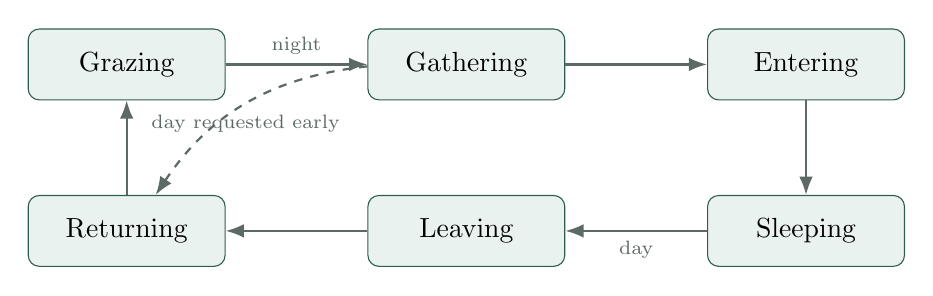
\begin{tikzpicture}[
			node distance=12mm and 18mm,
			st/.style={draw=FarmGreen,rounded corners,fill=FarmGreenLight,minimum width=25mm,minimum height=9mm,align=center},
			arr/.style={-{Latex},thick,Muted}
		]
		\node[st] (g) {Grazing};
		\node[st,right=of g] (ga) {Gathering};
		\node[st,right=of ga] (e) {Entering};
		\node[st,below=of e] (s) {Sleeping};
		\node[st,left=of s] (l) {Leaving};
		\node[st,left=of l] (r) {Returning};
		\draw[arr] (g)--node[above,font=\scriptsize]{night} (ga);
		\draw[arr] (ga)--(e);
		\draw[arr] (e)--(s);
		\draw[arr] (s)--node[below,font=\scriptsize]{day} (l);
		\draw[arr] (l)--(r);
		\draw[arr] (r)--(g);
		\draw[arr,dashed] (ga) to[bend right=25] node[below,font=\scriptsize]{day requested early} (r);
	\end{tikzpicture}
\end{center}

\section{Initial cows}
The herd contains three cows centered around approximately \code{\{9,0,10\}}, \code{\{16,0,12\}} and \code{\{9,0,18\}}, each with a different animation offset.

\section{Lane and queue}
The shared lane follows:
\begin{enumerate}
	\item pasture queue/gate near \code{\{7,0,15\}},
	\item \code{\{0,0,15\}},
	\item world center \code{\{0,0,0\}},
	\item \code{\{-17,0,0\}},
	\item barn aisle position.
\end{enumerate}
Queue spacing is 5 units. Herd route speed is 2.4 units/s.

\section{Night sequence}
When night is requested:
\begin{enumerate}
	\item Save each cow's field position.
	\item Sort cows by X so the lineup is stable.
	\item Walk them to queue positions X=7,12,17 at Z=15.
	\item Open barn doors.
	\item Advance the convoy toward the barn with spacing.
	\item Send one cow at a time from aisle to its own bed.
	\item Once all three are placed, close doors and enter Sleeping.
\end{enumerate}

\section{Morning sequence}
The exit is deliberately more cautious. Cows back out from stalls, rotate in the aisle, face the door and then follow the reverse route. The farthest queue member exits first so following cows remain separated.

\section{Status text}
The state machine still owns the behavior, but \code{Herd::status()} now returns localized catalog entries such as \code{herd.grazing}, \code{herd.entering}, \code{herd.leaving_night} and \code{herd.returning}. Rewording status messages therefore does not affect route logic.

\begin{warningbox}
	The Herd code is the most behavior-sensitive module. Small route changes can affect door safety, queue spacing and verification invariants. After editing it, always run \file{scripts/verify.ps1} rather than relying only on visual inspection.
\end{warningbox}

\chapter{Animation System}
\file{src/systems/AnimationSystem.h} is intentionally tiny:
\begin{lstlisting}[language=C++]
class AnimationSystem {
  public:
    bool paused = false;
    float time = 0;
    float update(float dt) {
        if (paused) return 0;
        time += dt;
        return dt;
    }
};
\end{lstlisting}
This creates a useful design: every animated system receives either the real delta or zero. Pausing therefore freezes wind time, windmill, herd, sky and cutting updates without each subsystem needing its own pause flag.

\chapter{Grass Cutting System}
\section{Activation condition}
Cutting works only if enabled and camera Y is below 2.6. This prevents the overhead camera from mowing grass beneath it.

\section{Cutting circle}
When active near the ground, the system draws a 64-segment yellow line loop at Y about 0.065 with radius \code{CUT_RADIUS}. It disables lighting and textures for the indicator and restores state afterwards.

\begin{editbox}
	There are three different values you may want to tune:
	\begin{itemize}
		\item \textbf{Cut radius}: \code{CUT_RADIUS} in \file{Constants.h}.
		\item \textbf{Maximum cutting camera height}: 2.6 in \file{GrassCuttingSystem.cpp}.
		\item \textbf{Remaining blade height}: .22 in \file{Grass.cpp}.
	\end{itemize}
	These control different behaviors; do not confuse them.
\end{editbox}

\part{Verification, Capture, Build and Development Tooling}

\chapter{Frame Capture}
\file{src/core/Capture.cpp} reads pixels from the OpenGL back buffer using \code{glReadPixels}, swaps RGB to BGR order and writes a 24-bit BMP header and pixel data directly.

This feature exists mainly for deterministic verification and screenshots. It avoids adding a separate image-writing dependency.

\begin{beginnerbox}
	BMP rows are padded to 4-byte boundaries. The code computes \code{stride = (width * 3 + 3) \& \textasciitilde3}; that rounds each 24-bit RGB row up to a multiple of four bytes.
\end{beginnerbox}

\chapter{Run Options and Self-Verification}
\section{Command-line options}
\file{src/core/Verification.h/.cpp} defines \code{RunOptions}. Supported switches include capture path, view preset, simulation time, wind, width/height, benchmark frames, self-test, night, morning, cut demo, no textures, wireframe, no HUD and no structural study.

\begin{longtable}{@{}lp{0.55\textwidth}@{}}
	\toprule
	Option                      & Purpose                                                                  \\
	\midrule
	\endhead
	\code{--capture PATH}       & Render and save a BMP frame, then exit.                                  \\
	\code{--view NAME}          & Select overview/meadow/crops/cows/cutting/barn and several side presets. \\
	\code{--time SECONDS}       & Advance simulation before capture.                                       \\
	\code{--wind VALUE}         & Set wind strength.                                                       \\
	\code{--width N --height N} & Set window/capture dimensions within validated limits.                   \\
	\code{--benchmark N}        & Render N frames and report FPS / OpenGL errors.                          \\
	\code{--self-test}          & Run behavior invariants and exit.                                        \\
	\code{--night}              & Request night before advancing.                                          \\
	\code{--morning}            & First settle into night, then request morning.                           \\
	\code{--cut-demo}           & Pre-cut a path through the meadow.                                       \\
	\code{--no-textures}        & Disable texture use.                                                     \\
	\code{--wireframe}          & Render polygon lines.                                                    \\
	\code{--no-hud}             & Hide all HUD overlays.                                                   \\
	\code{--no-study}           & Keep the HUD visible but hide the structural-study panel.                \\
	\bottomrule
\end{longtable}

\section{What the self-test checks}
The verification code checks, among other things:
\begin{itemize}
	\item Wind roots stay exactly fixed and quarter-height displacement follows the expected squared relation.
	\item Wind clamps between 0 and 3 and behaves consistently across update rates.
	\item Grass generation is deterministic and exactly 2800 blades.
	\item Cutting only affects nearby cuttable grass, cannot happen while flying, is idempotent and resets correctly.
	\item Camera movement follows yaw, respects minimum height/bounds and clamps pitch.
	\item All camera presets are valid; cycling and HUD toggles do not modify simulation state.
	\item The text catalog falls back to embedded defaults, accepts valid overrides, rejects malformed reloads without losing the previous catalog, and supports placeholders.
	\item Windmill rotation is frame-rate independent and stops at zero wind.
	\item Cows walk/graze appropriately.
	\item Herd line-up, door safety, single-file travel, sleeping placement and return behavior are correct.
\end{itemize}

\chapter{CMake Build System}
\section{Top-level configuration}
\file{CMakeLists.txt} requires CMake 3.21, requests C/C++, sets C++20, includes the FreeGLUT dependency helper, finds OpenGL, recursively collects \file{src/*.cpp} and \file{src/*.h}, and creates the executable.

\section{Linking}
The target links:
\begin{itemize}
	\item \code{freeglut\_static}
	\item \code{OpenGL::GL}
	\item \code{OpenGL::GLU}
\end{itemize}
It defines \code{NOMINMAX}, \code{FREEGLUT_STATIC} and \code{GLUT_DISABLE_ATEXIT_HACK}.

\section{Generated text fallback}
Before creating the target, CMake sets \code{FARM_TEXT_INPUT} to \file{assets/text.txt} and includes \file{cmake/EmbedText.cmake}. That script marks the text file as a configure dependency, reads it, checks that it does not contain the reserved raw-string delimiter, and configures \file{generated/TextDefaults.h}. The generated directory is added to the target include paths.

This is why the runtime can start with built-in labels even when the editable external text file is missing. The external file is still copied as part of \file{assets/} and remains the preferred editable source.

\section{Warnings}
MSVC builds use \code{/W4 /permissive-}. Other compilers use \code{-Wall -Wextra -Wpedantic}.

\section{Post-build copying}
CMake copies \file{assets/} beside the executable and copies FreeGLUT's license as \file{FREEGLUT-LICENSE.txt}.

\section{CTest}
Two tests are registered: \code{farm\_invariants} runs \code{--self-test}; \code{farm\_render} captures an overview BMP.

\chapter{Pinned FreeGLUT Dependency}
\file{cmake/FreeGLUT.cmake} uses CMake \code{FetchContent}. It requests FreeGLUT 3.8.0, disables demos/shared libraries, enables the static library, downloads from GitHub's codeload archive and verifies SHA-256:
\begin{lstlisting}
66c12fbf41ef5da34a386d59dbd389e30b601124937f8edb81a30a5006247f93
\end{lstlisting}

\begin{whybox}
	Pinning a version plus checksum improves reproducibility. A future FreeGLUT release cannot silently change the build, and a corrupted/tampered archive will fail checksum validation.
\end{whybox}

\chapter{Windows Build and Maintenance Scripts}
\section{\texttt{scripts/build.ps1}}
Finds Visual Studio with \code{vswhere.exe}, requires the x86/x64 C++ tools component, runs MSBuild on the project, and optionally executes \code{--self-test}. Defaults are Release/x64.

\section{\texttt{scripts/setup.ps1}}
Finds CMake directly or through Visual Studio, configures the dependency-only CMake project under \file{build/deps/<platform>} and builds \code{freeglut\_static}. This separates dependency preparation from the main Visual Studio project.

\section{\texttt{scripts/verify.ps1}}
Runs an extensive Release/x64 verification suite. It can skip rebuilding and can refresh the README screenshot. It captures many cases: overview, still/windy meadow, cutting, crops, night, barn entry, sleeping, morning, empty barn, side barn views, small window, no-HUD, no-study, front/back/left/right, cows, wireframe and no-textures. It also benchmarks 180 frames, tests native window shutdown, tests startup with no assets, and checks the editable text-file behavior.

\section{\texttt{scripts/test-shutdown.ps1}}
Starts the native executable, waits until its window exists, sends a real close request through \code{CloseMainWindow()}, checks timely process exit and rejects FreeGLUT errors such as \code{no current window}. This protects the timer/close edge case handled by \code{closing} in \file{main.cpp}.

\section{\texttt{scripts/sync-project.ps1}}
Rebuilds Visual Studio's source item list and Solution Explorer filters from the actual \file{src} directory and also includes \file{assets/text.txt} as a non-compiled project item. Use it after adding/removing C++ source/header files if Visual Studio's project view is out of sync.

\section{Formatting}
The project documentation describes \file{scripts/format.ps1} as orchestrating clang-format for C++, mdformat for Markdown, PSScriptAnalyzer for PowerShell, Ruff for Python, cmake-format for CMake and .NET XML rewriting for project XML. The owned-file set now explicitly includes \file{assets/text.txt} and \file{*.in} templates. Tools are cached under ignored build directories.

\chapter{Visual Studio Project Files and Editor Configuration}
The repository includes \file{csc3081\_farm\_project.slnx}, \file{csc3081\_farm\_project.vcxproj} and \file{.vcxproj.filters}. These support opening/building in Visual Studio while CMake remains another supported build path.

Root files \file{.clang-format} and \file{.editorconfig} standardize formatting/whitespace. \file{.gitattributes} and \file{.gitignore} control Git text handling and ignored build/editor outputs.

\begin{beginnerbox}
	The C++ source files are the product logic. Visual Studio project files are build/IDE metadata. Do not manually duplicate a newly created source file into several places: add it under \file{src/}, then run \file{scripts/sync-project.ps1} for Visual Studio metadata.
\end{beginnerbox}

\part{Customization Cookbook: Change the Farm Without Getting Lost}

\chapter{Master Parameter Map}
This chapter is the fastest reference for common edits.

\begin{longtable}{@{}p{0.24\textwidth}p{0.23\textwidth}p{0.14\textwidth}p{0.31\textwidth}@{}}
	\toprule
	What you want to change    & File / identifier                       & Current           & Notes                                                                                    \\
	\midrule
	\endhead
	Camera movement speed      & \file{Constants.h}: \code{CAMERA_SPEED} & 6.0               & Global free-camera speed.                                                                \\
	User-facing labels         & \file{assets/text.txt}                  & key/value catalog & Farm title, author, views, herd, help, signs, stalls and status wording; reload with F9. \\
	Lowest camera height       & \code{EYE_MIN}                          & 1.35              & Prevents going underground.                                                              \\
	Max wind                   & \code{WIND_MAX}                         & 3.0               & Used by clamp and UI assumptions.                                                        \\
	Cutting radius             & \code{CUT_RADIUS}                       & 1.8               & Also sizes yellow ring.                                                                  \\
	Grass smoothness           & \code{GRASS_SEGMENTS}                   & 5                 & Higher = more triangles.                                                                 \\
	Grass total count          & \file{Grass.cpp} loop                   & 2800              & First 2300 are meadow/cuttable.                                                          \\
	Cut grass remaining height & \file{Grass.cpp}                        & 0.22x             & Fraction of original.                                                                    \\
	Cutting max camera Y       & \file{GrassCuttingSystem.cpp}           & 2.6               & Above this, cutting is disabled.                                                         \\
	Default wind strength      & \file{WindSystem.h}                     & 1.2               & Starting scene state.                                                                    \\
	Wind wave speed            & \file{WindSystem.h}                     & 2.2               & Time frequency multiplier.                                                               \\
	Global bend scale          & \file{WindSystem.cpp}                   & 0.32              & Multiplied by plant height/flexibility.                                                  \\
	Windmill spin scale        & \file{Windmill.cpp}                     & 65                & Degrees/s per wind-strength unit.                                                        \\
	Sky transition rate        & \file{Sky.cpp}                          & 0.4               & Full fade about 2.5 s.                                                                   \\
	Cloud drift                & \file{Sky.cpp}                          & 0.25              & X units/second factor.                                                                   \\
	Barn door rate             & \file{Barn.cpp}                         & 0.65              & Open/close normalized units per second.                                                  \\
	Herd route speed           & \file{Herd.cpp}                         & 2.4               & Keep aligned with cow walk speed if desired.                                             \\
	Herd queue gap             & \file{Herd.cpp}                         & 5                 & Single-file spacing.                                                                     \\
	Cow field route radius     & \file{Cow.cpp}                          & 2.1               & Circular wandering radius.                                                               \\
	Cow leg walk frequency     & \file{Cow.cpp}                          & 4.5 / 7           & Field/route leg oscillation.                                                             \\
	Perspective FOV            & \file{main.cpp}: \code{gluPerspective}  & 55 deg            & Lens angle.                                                                              \\
	Mouse sensitivity          & \file{main.cpp}: \code{motion}          & 0.2               & Degrees per pixel.                                                                       \\
	Timer target interval      & \file{main.cpp}                         & 16 ms             & Roughly 60 Hz updates.                                                                   \\
	\bottomrule
\end{longtable}

\chapter{Changing Colors}
\section{Rules of thumb}
Colors are usually \code{Vec3} values or direct \code{glColor3f}. Search within the target module for three floating-point values in braces or \code{glColor3f}. Examples:

\begin{longtable}{@{}p{0.25\textwidth}p{0.34\textwidth}p{0.33\textwidth}@{}}
	\toprule
	Object          & Current approximate color           & File                           \\
	\midrule
	\endhead
	Barn wall       & \rgb{.66}{.23}{.17}                 & \file{structures/Barn.cpp}     \\
	Barn trim       & \rgb{.94}{.86}{.67}                 & \file{structures/Barn.cpp}     \\
	Windmill timber & \rgb{.42}{.32}{.22}                 & \file{structures/Windmill.cpp} \\
	Fence wood      & \rgb{.64}{.48}{.29}                 & \file{structures/Fence.cpp}    \\
	Hay             & \rgb{.82}{.64}{.25}                 & \file{objects/HayBale.cpp}     \\
	Cow white       & \rgb{.92}{.89}{.77}                 & \file{animals/Cow.cpp}         \\
	Cow black       & \rgb{.16}{.19}{.17}                 & \file{animals/Cow.cpp}         \\
	Cow pink        & \rgb{.75}{.49}{.40}                 & \file{animals/Cow.cpp}         \\
	Grass           & gradient around \rgb{.32}{.49}{.16} & \file{vegetation/Grass.cpp}    \\
	Crop stalk      & \rgb{.58}{.57}{.20}                 & \file{vegetation/Crop.cpp}     \\
	Tree trunk      & \rgb{.39}{.27}{.16}                 & \file{vegetation/Tree.cpp}     \\
	HUD panel       & \rgb{.075}{.14}{.13}, alpha .82     & \file{core/Hud.cpp}            \\
	\bottomrule
\end{longtable}

\section{Example: make the barn blue}
In \file{Barn.cpp}, change the local \code{red} vector from something like \code{\{.66f,.23f,.17f\}} to, for example, \code{\{.20f,.38f,.68f\}}. Rebuild and check day and night views because lighting changes perceived color.

\section{Why texture and color can both matter}
When texturing is enabled with \code{GL\_MODULATE}, texture color is multiplied by the current material/color. This means a dark \code{glColor3f} can darken a bright texture. If a texture seems unexpectedly tinted, inspect both the bound texture and current color.

\chapter{Changing Positions, Sizes and Shapes}
\section{Position vectors}
Most whole-object placement happens with either a center argument or \code{glTranslatef}. Change X/Z to move along the ground and Y to raise/lower.

\section{Dimensions}
For \code{Draw::box(center,size,color)}, \code{size.x} is width, \code{size.y} is height and \code{size.z} is depth. For \code{Draw::ellipsoid(center,size,color)}, the size values are scale/radius-like factors along each axis.

\section{Safe and risky moves}
\begin{tabularx}{\textwidth}{@{}lXX@{}}
	\toprule
	Risk   & Examples                              & Why                                                                \\
	\midrule
	Low    & Rock, hay bale, decorative tree, sign & Few/no other systems depend on coordinates.                        \\
	Medium & Windmill, trough, crop field extents  & May overlap paths/fences but no route logic.                       \\
	High   & Barn, pasture gate, central paths     & Herd routes, camera views, fences and verification depend on them. \\
	\bottomrule
\end{tabularx}

\chapter{Changing Movement and Animation}
\section{Camera}
Change \code{CAMERA_SPEED}; arrow-look speed is 65 deg/s yaw and 55 deg/s pitch in \file{Camera.cpp}; right-drag sensitivity is 0.2 deg/pixel in \file{main.cpp}.

\section{Wind}
Use default strength, max strength, time speed, direction, global bend scale and per-plant flexibility/frequency.

\section{Windmill}
The rotor uses \code{strength * 65 * dt}. Keep \code{fmod(...,360)} so the angle does not grow without bound.

\section{Cow and herd}
The individual cow route and the herd's path-following use related but separate values. If you globally want faster cows, update both and rerun verification.

\section{Day/night}
Sky visual fade and herd behavior trigger are conceptually separate. \code{sky.night} immediately changes the requested behavioral state, while \code{nightAmount} visually eases over time.

\chapter{Changing Grass and Crops}
\section{More/less grass}
Change total loop count and meadow count. Keep meadow count \(\le\) total count. The HUD now reports the current cut count without a hardcoded \code{/ 2300} total, so changing the meadow count no longer requires a matching HUD literal edit.

\section{Grass density versus performance}
Every additional blade adds \code{GRASS_SEGMENTS * 2} triangles. Doubling blades roughly doubles grass geometry work. Reducing segments from 5 to 3 lowers geometry cost but makes bending visibly more angular.

\section{Crop spacing}
The crop generator and terrain furrow generator both use approximately 1.15 X spacing. Change them together.

\chapter{Changing the Barn and Cow Routine}
\section{Change stall spacing}
Current stall centers are separated by 1.5 in X. That value appears in both \code{Barn::aisle()} and \code{Barn::bed()}, and stall geometry in \file{Barn.cpp} uses the same spacing. Change all related expressions together.

\section{Change number of cows}
This is \textbf{not} a one-line edit. The current Herd uses fixed \code{std::array<...,3>} structures, loops with 3, three stall beds, and verification expectations. The HUD count is formatted dynamically, but the simulation itself is still structurally three-cow. Converting to N cows requires a deliberate refactor to dynamic or templated sizes.

\begin{warningbox}
	If you want four cows, do not only add a fourth \code{Cow} constructor. You must also add a fourth stall or define sharing behavior, generalize arrays/loop bounds, queue order, exit rules and verification. You may also want to adjust wording in \file{assets/text.txt}, but the visible numeric sleep count itself is already formatted at runtime.
\end{warningbox}

\chapter{Changing HUD Text, Sign Text and Author Metadata}
\section{One source of truth}
The preferred place for user-facing wording is now \file{assets/text.txt}. Change the value after \code{=} and keep the key unchanged. Save the file and press \keycap{F9}; the application attempts to reload it without rebuilding.

\section{Author, registration and farm title}
Edit \code{farm.author} and \code{farm.title}. The old \code{AUTHOR_NAME} and \code{REGISTRATION_NUMBER} constants were removed from \file{Constants.h}.

\section{Camera and herd wording}
Edit \code{view.*} and \code{herd.*}. The camera and herd state machine now resolve these labels through the text catalog, so wording changes do not touch movement/behavior code.

\section{World signs and stalls}
Edit \code{sign.meadow}, \code{sign.meadow_hint}, \code{sign.pasture}, \code{sign.wheat} and \code{stall.1..3}. For example, \code{stall.1 = Buttercup} immediately renames the first plaque after an F9 reload.

\section{Controls, wind and structural-study wording}
Edit \code{help.*}, \code{wind.*}, \code{study.*} and \code{cutting.*}. Keep placeholders such as \code{\{value\}}, \code{\{maximum\}}, \code{\{mode\}} and \code{\{count\}} intact when they appear.

\section{Window title is separate}
The native window caption \code{"CSC3081 | Interactive 3D Farm"} still lives in \file{main.cpp}. Changing \code{farm.title} affects the HUD, not the operating-system window title or README heading.

\begin{warningbox}
	If F9 reports a failure, check for a missing \code{=}, empty key/value, non-ASCII character in a value, overly long line, or damaged placeholder/key. The loader keeps the previous valid catalog when a reload fails.
\end{warningbox}

\chapter{Changing or Replacing Textures}
\section{Drop-in replacement}
The safest method is to preserve the same file name, location and 24-bit uncompressed BMP format. Keep a modest power-of-two size such as 64x64 or 128x128.

\section{Add a fifth texture type}
You must:
\begin{enumerate}
	\item Add an enum item before \code{Count} in \file{Texture.h}.
	\item Increase/update the ID array size or derive it from \code{Count}.
	\item Add a path in \code{TextureSet::initialize()} matching enum order.
	\item Bind that surface before drawing the target object.
	\item Add/copy the asset in the runtime \file{assets} tree.
\end{enumerate}

\chapter{Adding a New Object Module}
Suppose you want a tractor.
\section{1. Create files}
Create \file{src/objects/Tractor.h} and \file{Tractor.cpp}. Give the class a \code{render() const} method.

\begin{lstlisting}[language=C++]
#pragma once
class Tractor {
  public:
    void render() const;
};
\end{lstlisting}

\section{2. Build from existing primitives}
Use \code{Draw::box}, \code{Draw::ellipsoid} and transforms. Start with simple shapes before adding detail.

\section{3. Add it to Scene}
Include the header in \file{Scene.h}, add a \code{Tractor tractor;} member, then call \code{tractor.render();} in a sensible place in \code{Scene::render()}.

\section{4. Sync Visual Studio metadata}
CMake's recursive source glob will see the files. For the Visual Studio project, run \file{scripts/sync-project.ps1}.

\section{5. Verify}
Build, inspect multiple camera views, run self-test and full verification. A purely visual tractor may not require new tests, but it must not create OpenGL errors.

\chapter{Adding a New Keyboard Toggle}
Example: toggle a tractor visibility flag.
\begin{enumerate}
	\item Add a boolean member to \code{Scene}, such as \code{bool showTractor = true;}.
	\item In \code{Scene::key}, add \code{if (key == 'x') showTractor = !showTractor;}.
	\item In render, wrap tractor drawing in \code{if (showTractor)}.
	\item Add help text in the HUD.
	\item Update README controls and verification if the feature matters to required behavior.
\end{enumerate}

\begin{warningbox}
	Choose a key that is not already used. Remember \code{main.cpp} lowercases ordinary input before sending it to \code{Scene::key}.
\end{warningbox}

\chapter{Adding a New Camera View}
The current enum contains eight actual views plus \code{Count}. To add one:
\begin{enumerate}
	\item Add an enum item before \code{Count}.
	\item Add its position/target in \code{Camera::setView()}.
	\item Add its name in \code{viewName()}.
	\item Decide how users select it. F1--F8 are already mapped and the current special-key logic assumes that range.
	\item Update cycling, HUD help, README and verification.
\end{enumerate}

\begin{beginnerbox}
	A simpler alternative is to add a letter shortcut that directly sets \code{camera.position}, \code{yaw} and \code{pitch}, similar to the verification-only crop/cow camera presets. That avoids changing the enum/F-key design.
\end{beginnerbox}

\part{Debugging and Learning Guides}

\chapter{How to Read an OpenGL Object Function}
When you open a render function, use this checklist:
\begin{enumerate}
	\item Find outer \code{glPushMatrix}/\code{glPopMatrix}. This defines the object's local transform scope.
	\item Find \code{glTranslatef}: likely whole-object position.
	\item Find \code{glScalef}: likely whole-object or subpart size.
	\item Find loops: repeated posts, blades, leaves, legs, rails, straw, etc.
	\item Find colors: \code{Vec3} constants or \code{glColor3f}.
	\item Find helper calls: \code{box}, \code{beam}, \code{ellipsoid}, \code{ground}, \code{triangle}.
	\item Find nested push/pop blocks: articulated subparts such as windmill blades or cow legs.
\end{enumerate}

\chapter{Common Problems and How to Diagnose Them}
\section{Black or untextured surfaces}
Press \keycap{T} to compare with textures off. Check asset paths and BMP format. The runtime prints a warning if a texture cannot load.

\section{Object moved unexpectedly}
Look for a missing \code{glPopMatrix()} or a transform placed outside the intended push/pop scope.

\section{Object is too dark}
Toggle lighting with \keycap{L}. Check normals and the current color. With texturing in modulate mode, dark colors also darken textures.

\section{Camera enters ground}
Check \code{EYE_MIN} and Y clamp in \file{Camera.cpp}. Do not set preset positions below the minimum.

\section{Cows do not enter barn}
Inspect barn door opening state, \code{passable()}, lane coordinates, \code{Barn::aisle()} and \code{Barn::bed()}. Run \code{--self-test} for a precise failure label.

\section{Grass cuts while flying or does not cut}
Check cutting enabled flag, camera Y threshold 2.6 and \code{CUT_RADIUS}. Use meadow view \keycap{G} to reach ground level.

\section{Program crashes on close}
Do not remove the \code{closing} guards casually. The code explicitly accounts for outstanding GLUT timer callbacks around window destruction, and \file{test-shutdown.ps1} verifies this behavior.

\chapter{Recommended Beginner Editing Workflow}
\begin{enumerate}
	\item Build and run the unchanged project once.
	\item Pick one visible target (for example barn color).
	\item Search the handbook for that target's module.
	\item Make one small change.
	\item Build and inspect from at least overview + one close view.
	\item Run \code{--self-test}; for structural/behavior changes run \file{scripts/verify.ps1}.
	\item Commit the small change before starting another category.
\end{enumerate}

\begin{whybox}
	Small commits make graphics experimentation much safer. If one set of coordinate changes breaks the scene, you can compare or revert just that edit instead of untangling five unrelated experiments.
\end{whybox}

\chapter{Suggested Refactors for Easier Future Customization}
The current project is readable, but many visual values are embedded directly in render functions. If this project will be edited frequently, consider these refactors.

\section{Central theme colors}
Create a \file{Theme.h} containing named colors such as \code{BarnRed}, \code{WoodDark}, \code{GrassBase}. This makes global recoloring easy.

\section{Scene layout constants}
Create \file{FarmLayout.h} for barn center, windmill center, pasture bounds, gate position and crop field bounds. Herd, camera and render modules could then share one source of truth.

\section{Configuration structs}
Represent tree placements, hay bales, signs and camera presets as arrays of structs rather than repeated calls. That reduces copy/paste errors.

\section{Derive fixed counts}
Replace remaining hardcoded \code{3} cow/stall references with values derived from containers/configuration where reasonable. The previous hardcoded \code{2300} HUD total has already been removed, and user-facing wording has already moved to \file{assets/text.txt}.

\section{Modern OpenGL path}
For coursework demonstrating immediate mode, the current approach is understandable. For a larger project, batching geometry into vertex buffers, using shaders and instance rendering would improve scalability. This is an architectural migration, not a beginner customization.

\appendix
\part{Reference Appendices}

\chapter{Complete C++ Source File Index}
\begin{longtable}{@{}p{0.36\textwidth}p{0.56\textwidth}@{}}
	\toprule
	File & Role \\
	\midrule
	\endhead
	\pathrow{src/main.cpp}{Entry point, GLUT callbacks, timing, input, window lifecycle, capture and benchmark orchestration.}
	\pathrow{src/animals/Cow.h}{Cow interface and animation state.}
	\pathrow{src/animals/Cow.cpp}{Field cycle, path walking, heading, sleep transition, cow geometry and catalog-backed sleep symbol.}
	\pathrow{src/core/Camera.h}{Camera state and view enum.}
	\pathrow{src/core/Camera.cpp}{Movement, look, projection view transform and camera presets.}
	\pathrow{src/core/Capture.h}{Frame capture declaration.}
	\pathrow{src/core/Capture.cpp}{OpenGL framebuffer to BMP writer.}
	\pathrow{src/core/Hud.h}{HUD state structure and renderer interface.}
	\pathrow{src/core/Hud.cpp}{Scale-aware edge overlays, localized status/help/wind panels and structural-study diagram.}
	\pathrow{src/core/Lighting.h}{Lighting interface.}
	\pathrow{src/core/Lighting.cpp}{Global fixed-function light setup.}
	\pathrow{src/core/Scene.h}{Top-level scene ownership and public scene API.}
	\pathrow{src/core/Scene.cpp}{Initialization, simulation update order, keyboard toggles, F9 text reload notice and render order.}
	\pathrow{src/core/Text.h}{TextCatalog interface plus initialize/reload/get/format API.}
	\pathrow{src/core/Text.cpp}{Editable key/value parser, embedded defaults, path resolution, reload safety and placeholder formatting.}
	\pathrow{src/core/Texture.h}{Texture surface enum and loader/binder interface.}
	\pathrow{src/core/Texture.cpp}{24-bit BMP validation/loading, mipmaps and runtime binding.}
	\pathrow{src/core/Verification.h}{Run options and verification interface.}
	\pathrow{src/core/Verification.cpp}{CLI parsing, deterministic presets and behavior invariants.}
	\pathrow{src/environment/Path.h}{Path renderer interface.}
	\pathrow{src/environment/Path.cpp}{Path rectangles and catalog-backed world signs.}
	\pathrow{src/environment/Sky.h}{Day/night target and transition state.}
	\pathrow{src/environment/Sky.cpp}{Sky color transition, moving clouds and bright celestial body.}
	\pathrow{src/environment/Terrain.h}{Terrain renderer interface.}
	\pathrow{src/environment/Terrain.cpp}{Farm base, grass zones, dirt and crop furrows.}
	\pathrow{src/objects/HayBale.h}{Hay-bale helper and object renderer.}
	\pathrow{src/objects/HayBale.cpp}{Hay geometry, outdoor bale placement and water trough.}
	\pathrow{src/objects/Rock.h}{Rock renderer interface.}
	\pathrow{src/objects/Rock.cpp}{Procedural edge rock placement and dodecahedron rendering.}
	\pathrow{src/structures/Barn.h}{Barn door state, stall coordinate helpers and render/light interface.}
	\pathrow{src/structures/Barn.cpp}{Barn geometry, doors, stalls, hay, catalog-backed plaques and lamp.}
	\pathrow{src/structures/Fence.h}{Fence renderer and segment helper.}
	\pathrow{src/structures/Fence.cpp}{Fence post/rail generation, perimeter and pasture boundaries.}
	\pathrow{src/structures/Windmill.h}{Windmill rotor state.}
	\pathrow{src/structures/Windmill.cpp}{Wind-driven rotation and tower/blade geometry.}
	\pathrow{src/systems/AnimationSystem.h}{Pause-aware shared simulation time.}
	\pathrow{src/systems/GrassCuttingSystem.h}{Cutting toggle/update/render interface.}
	\pathrow{src/systems/GrassCuttingSystem.cpp}{Ground-height cut condition and yellow radius indicator.}
	\pathrow{src/systems/Herd.h}{Herd phases, three cows and route state.}
	\pathrow{src/systems/Herd.cpp}{Queueing, barn entry, sleep, exit and return state machine plus catalog-backed status messages.}
	\pathrow{src/systems/WindSystem.h}{Wind state, direction and deformation API.}
	\pathrow{src/systems/WindSystem.cpp}{Gust/wave formula and height-squared bending.}
	\pathrow{src/utils/Constants.h}{Shared numeric camera/wind/cutting/grass constants; text metadata moved to assets/text.txt.}
	\pathrow{src/utils/Font.h}{Custom font API.}
	\pathrow{src/utils/Font.cpp}{Atlas loading, text width, textured text and fallback stroke font.}
	\pathrow{src/utils/FontMetrics.h}{Generated printable-ASCII glyph advances.}
	\pathrow{src/utils/Helpers.h}{Drawing helper declarations.}
	\pathrow{src/utils/Helpers.cpp}{Box, ellipsoid, beam, ground, triangle, text, plaque and sign helpers.}
	\pathrow{src/utils/MathUtils.h}{Vec3 and vector/math helpers.}
	\pathrow{src/vegetation/Crop.h}{Crop stalk data and interface.}
	\pathrow{src/vegetation/Crop.cpp}{Procedural wheat rows and wind-deformed stalk/leaf/head geometry.}
	\pathrow{src/vegetation/Grass.h}{Grass blade data, render, cut/reset API.}
	\pathrow{src/vegetation/Grass.cpp}{Deterministic blade generation, segmented bending, cutting and reset.}
	\pathrow{src/vegetation/Tree.h}{Tree renderer interface.}
	\pathrow{src/vegetation/Tree.cpp}{Trunk, branches, foliage, leaves and placements.}
	\bottomrule
\end{longtable}

\chapter{Non-C++ Repository File Index}
\begin{longtable}{@{}p{0.42\textwidth}p{0.50\textwidth}@{}}
	\toprule
	File/path & Role \\
	\midrule
	\endhead
	\pathrow{README.md}{Project overview, build instructions, controls and development notes.}
	\pathrow{CMakeLists.txt}{Main CMake build, linking, generated text fallback include path, asset copy and tests.}
	\pathrow{assets/text.txt}{Editable shared user-facing labels; reload at runtime with F9.}
	\pathrow{cmake/FreeGLUT.cmake}{Pinned/checksummed FreeGLUT 3.8.0 FetchContent setup.}
	\pathrow{cmake/EmbedText.cmake}{Reads assets/text.txt and configures the generated embedded fallback header.}
	\pathrow{cmake/TextDefaults.h.in}{Raw-string template used to generate TextDefaults.h in the build tree.}
	\pathrow{cmake/dependencies/CMakeLists.txt}{Small dependency-only project used by setup script.}
	\pathrow{csc3081\_farm\_project.slnx}{Visual Studio solution.}
	\pathrow{csc3081\_farm\_project.vcxproj}{MSBuild C++ project.}
	\pathrow{csc3081\_farm\_project.vcxproj.filters}{Solution Explorer folder mapping.}
	\pathrow{scripts/build.ps1}{MSBuild wrapper + optional self-test.}
	\pathrow{scripts/setup.ps1}{FreeGLUT dependency setup/build.}
	\pathrow{scripts/verify.ps1}{Behavior/render/benchmark/shutdown/missing-asset verification suite.}
	\pathrow{scripts/test-shutdown.ps1}{Repeated native title-bar close testing.}
	\pathrow{scripts/sync-project.ps1}{Regenerates Visual Studio source entries and filters.}
	\pathrow{scripts/format.ps1}{Multi-language formatter/checker orchestration.}
	\pathrow{scripts/format-requirements.txt}{Pinned Python formatter requirements.}
	\pathrow{scripts/generate-textures.py}{Procedural generation of four BMP material textures.}
	\pathrow{scripts/generate-font.py}{Downloads/checks Patrick Hand, creates font atlas and metrics.}
	\pathrow{docs/SCRIPTS.md}{Usage reference for build, verify, formatting, text reload and generation scripts.}
	\pathrow{docs/CODE_WALKTHROUGH.md}{Repository-maintained beginner walkthrough covering code flow, tuning and common modification recipes.}
	\pathrow{docs/THIRD\_PARTY.md}{FreeGLUT and Patrick Hand attribution/license/reference notes.}
	\pathrow{assets/fonts/handwriting.bmp}{Runtime custom font atlas.}
	\pathrow{assets/fonts/OFL.txt}{SIL Open Font License for Patrick Hand-derived atlas.}
	\pathrow{assets/textures/terrain/grass\_ground.bmp}{Ground material texture.}
	\pathrow{assets/textures/terrain/dirt.bmp}{Dirt material texture.}
	\pathrow{assets/textures/structures/wood.bmp}{Wood material texture.}
	\pathrow{assets/textures/structures/hay.bmp}{Hay material texture.}
	\pathrow{screenshots/overview.png}{README/project overview screenshot.}
	\pathrow{.clang-format}{C++ formatting rules.}
	\pathrow{.editorconfig}{Cross-editor indentation/encoding/whitespace settings.}
	\pathrow{.gitattributes}{Git attribute/text behavior configuration.}
	\pathrow{.gitignore}{Ignored generated build/editor artifacts.}
	\bottomrule
\end{longtable}

\chapter{Control Reference}
\begin{longtable}{@{}ll@{}}
	\toprule
	Input              & Action                                  \\
	\midrule
	\endhead
	W / A / S / D      & Move camera                             \\
	Arrow keys         & Look around                             \\
	Right mouse drag   & Look around                             \\
	Q / E              & Lower / raise camera                    \\
	G                  & Meadow view                             \\
	V                  & Overview                                \\
	H                  & Barn interior                           \\
	Tab                & Cycle eight camera views                \\
	F1                 & Overview                                \\
	F2 / F3            & Farm front / back                       \\
	F4 / F5            & Farm left / right                       \\
	F6 / F7 / F8       & Barn center / left / right              \\
	F9                 & Reload shared text from assets/text.txt \\
	F10                & Hide/show all overlays                  \\
	+ or = / -         & Increase/decrease wind                  \\
	0 / 1 / 2 / 3      & Wind off/low/medium/strong              \\
	C                  & Toggle cutting                          \\
	R                  & Restore grass                           \\
	P                  & Pause/resume animation                  \\
	N                  & Toggle day/night request                \\
	B                  & Toggle structural-study overlay         \\
	L                  & Toggle lighting                         \\
	T                  & Toggle textures                         \\
	F                  & Toggle wireframe                        \\
	Esc / window close & Exit                                    \\
	\bottomrule
\end{longtable}

\chapter{Build and Verification Command Cheatsheet}
\begin{lstlisting}
# Visual Studio/MSBuild path
.\scripts\build.ps1 -Configuration Release
.\build\x64\Release\csc3081_farm_project.exe

# Build and immediately run self-test
.\scripts\build.ps1 -Configuration Release -Platform x64 -Test

# Full verification suite
.\scripts\verify.ps1

# Reuse existing build
.\scripts\verify.ps1 -SkipBuild

# Refresh README overview screenshot while verifying
.\scripts\verify.ps1 -SkipBuild -RefreshScreenshots

# CMake path
cmake -S . -B build/cmake -A x64
cmake --build build/cmake --config Release --parallel
.\build\cmake\Release\csc3081_farm_project.exe

# Format / formatting check
.\scripts\format.ps1
.\scripts\format.ps1 -Check
\end{lstlisting}

\chapter{Practical Change Checklist}
Before committing a visual or behavior change, ask:
\begin{itemize}
	\item Did I modify only the module I intended?
	\item Did I preserve push/pop OpenGL state around local transforms?
	\item If I changed a shared coordinate, did I update dependent routes/cameras?
	\item If I changed a fixed count, is that count hardcoded in the HUD, arrays or tests?
	\item If I changed texture files, are they still supported 24-bit BMPs?
	\item Does it look correct in day and night?
	\item Does it look correct with textures on and off?
	\item Does it look correct from overview and a close camera view?
	\item Does \code{--self-test} pass?
	\item For structural/behavior changes, does \file{scripts/verify.ps1} pass?
\end{itemize}

\chapter*{Closing Mental Model}
\addcontentsline{toc}{chapter}{Closing Mental Model}
Willowfield becomes much simpler once you separate \textbf{where state changes} from \textbf{where geometry is drawn}. \file{main.cpp} drives the loop. \code{Scene} connects the world. Small systems own behaviors. Render modules translate positions, colors and dimensions into OpenGL primitives. \file{assets/text.txt} now owns most user-facing wording, while \code{Text.*} safely loads and formats it. Utilities keep repeated math and drawing code in one place. The verification suite protects important behavior while you experiment.

For most appearance edits, you can safely work in one render module and use the cookbook tables. For behavior edits, trace the update path and identify every module that shares the relevant state. That habit---following data instead of guessing from visuals---is the main skill that makes this codebase editable rather than mysterious.

\vfill
\begin{center}
	\color{Muted}\small
	\textbf{Documentation snapshot used by this handbook}\\[0.18cm]
	\href{https://github.com/Sivothajan/csc3081_farm_project/tree/de29e8f8a2b92f47097514f5d0ad8c3b512e058d}{\texttt{Sivothajan/csc3081\_farm\_project @ de29e8f}}\\
	Main branch state recorded on 7 September 2026.
\end{center}

\end{document}
